%%%%%%%%%%%%%%%%%%%%%%%%%%%%%%%%%%%%%%%%%
% baposter Portrait Poster
% LaTeX Template
% Version 1.0 (15/5/13)
%
% Created by:
% Brian Amberg (baposter@brian-amberg.de)
%
% This template has been downloaded from:
% http://www.LaTeXTemplates.com
%
% License:
% CC BY-NC-SA 3.0 (http://creativecommons.org/licenses/by-nc-sa/3.0/)
%
%%%%%%%%%%%%%%%%%%%%%%%%%%%%%%%%%%%%%%%%%

%----------------------------------------------------------------------------------------
%	PACKAGES AND OTHER DOCUMENT CONFIGURATIONS
%----------------------------------------------------------------------------------------

\documentclass[a0paper,portrait, fontscale=0.30]{baposter}
%\documentclass[a0paper,portrait,fontscale=0.345]{baposter}

\usepackage[utf8]{inputenc}
\usepackage{amssymb,amsbsy,amsmath,amsfonts,amssymb,amscd,amsthm}
%\usepackage[font=small,labelfont=bf]{caption} % Required for specifying captions to tables and figures
\usepackage[font=small,labelfont=bf,skip=2pt]{caption}
\usepackage{graphicx,subcaption}
\usepackage{subfig}
\usepackage{float}

\usepackage{comment} 
\usepackage{enumitem}
\usepackage{multirow}
\usepackage{verbatim}
\setlength{\floatsep}{10pt plus 1.0pt minus 2.0pt}
\usepackage{algorithmicx}
\usepackage{algpseudocode}
%\usepackage{relsize} % Used for making text smaller in some places
%\usepackage{empheq}
%% ------
%% COLORS
%% ------
\usepackage{transparent}
\definecolor{lightblue}{rgb}{0.145,0.6666,1}

% -------------
% Define colors
\definecolor{ceatitle}{rgb}{0.4, 0.4, 0.4}	%gris
\definecolor{ceaframetitle}{rgb}{1, 1, 1}	%blanc
\definecolor{ceagreen}{rgb}{0.58, 0.76, 0.11}
\definecolor{ceared}{rgb}{0.88, 0, 0.1}
\definecolor{ceablue}{rgb}{0.20, 0.47, 1}
%\definecolor{myred}{red}{0.6}
%-------------
% CEA THEME
%-------------

\renewcommand\labelitemi{
\includegraphics[scale=0.035]{item}}



\graphicspath{{../img/}} % Directory in which figures are stored


% box in box %not used
%\usepackage[framemethod=tikz,xcolor=true]{mdframed}
%
%\newmdenv[%		%block inside box
%    %leftmargin=0.cm,
%    %backgroundcolor=yellow!10,%
%    roundcorner=5pt,%
%    tikzsetting={draw=lightblue, line width=1.pt}%
%    ]{SpecialText}%

\usepackage{tcolorbox}
\newtcbox{\mybox}{%
	nobeforeafter,
	opacityframe=1,
	opacityback=1,
	colback=white,
	boxrule=0.02pt,
	minipage,
	width=0.02\linewidth,
	height=1cm,%5cm
	arc=1pt,
	boxsep=0pt,
	colframe=lightblue
  }

\begin{document}

\begin{poster}
{  
            % Options
            % Show grid to help with alignment
            grid=false,
            % Column spacing
            colspacing=0.4em,
            % Color style
            bgColorOne=white,
            bgColorTwo=white,
            borderColor=lightblue,		% Border color of content boxes
            headerColorOne=ceared!60!black, 		% Background color for the header in the content boxes (left side)
            headerColorTwo=ceared,	% Background color for the header in the content boxes (right side)
            headerFontColor=white,		% Text color for the header text in the content boxes
            boxColorOne=white, 		% Background color for the content in the content boxes
            % Format of textbox
            textborder=roundedleft,
            % Format of text header
            eyecatcher=true,
           	headerborder=none,		% Change to closed for a line under the content box headers
            headerheight=0.12\textheight,
            %textfont=\sc, An example of changing the text font
            headershape=roundedright,	% Specify the rounded corner in the content box headers
            headershade=shadelr,
            headerfont=\Large\bf\textsc, %Sans Serif	% Font modifiers for the text in the content box headers
            textfont={\setlength{\parindent}{1.00em}},%1.35em
            boxshade=plain,
            %background=shade-tb,
            background=plain,
            linewidth=1.0pt,%1.7
            columns=2
}
{
\includegraphics[scale=0.3]{logo_cea}}
{\transparent{0.5} \textcolor{red}{\Large \hspace{33pt} \center{Programme Transversal de Compétences Simulation Numérique}
\newline
}
\transparent{1.0} QUAD-BLOCKING%: Automatic generation of block-structured quadrilateral meshes
%Automatic generation of block-structured quadrilateral \\ \medskip meshes: singularity graph extraction
\vspace{0.1cm}
}
{% Poster Authors 
Ana-Maria \textsc{Vintescu}$^{1}$, 
Franck \textsc{Ledoux}$^{1}$,     
Francis \textsc{Kloss}$^{2}$,
Thibaud \textsc{Fortuna}$^{3}$,
Vincent \textsc{Bergeaud}$^{3}$\\
\smallskip
\small
 % $~^1$ smt else\\
%\smallskip
  $~^1$ CEA, DAM, DIF, F-91297 Arpajon, France \hspace{2em}  
  $~^2$ CEA, DEN, DM2S, 91400 Saclay, France \hspace{2em}  
  $~^3$ CEA, DRT, LIST, 91191 Gif-sur-Yvette, France \hspace{2em}
}
{
\includegraphics[scale=0.3]{logo_cea_list}} % logo-cea-list
%----------------------------------------------------------------------------------------
%	Context
%----------------------------------------------------------------------------------------
%%%%%%%%%%%%%%%%%%%%%%%%%%%%%%%%%%%%%%%%%%%%%%%%%%%%%%%%%%%%%%%%%%%%%
\vspace{-0.5cm}
\headerbox{Context}{name=context,column=0,row=0,span=2}{
%
%%%%%%%%%%%%%%%%%%%%%%%%%%%%%%%%%%%%%%%%%%%%%%%%%%%%%%%%%%%%%%%%%%%% 
\noindent
\begin{minipage}[b]{1.0\linewidth}
\vspace{-0.1cm}
\noindent
\begin{tcolorbox}[colframe=gray,boxrule=0.0pt,colback=lightgray]
\vspace{-0.1cm}
$\ \ \ \ \ \ \ \ \ \ \ \ \ \ \bullet$ Selection year of the project: 2018 $\ \ \ \ \ \ \ \ \ \ \ \ \ \ \bullet$ Starting date of the project: 28.01.2019 $\ \ \ \ \ \ \ \ \ \ \ \ \ \ \bullet$ duration of the project: 1 year$\ \ \ \ \ \ \ \ \ \ \ \ \ \ $%]
\vspace{-0.1cm}
\end{tcolorbox}
\vspace{-0.1cm}
\end{minipage}
\newline
\begin{minipage}[b]{0.4\linewidth}
Having available a high-order method for fast simulations on quadrilaterals(2D) and hexahedra(3D) $^{*}$,
perform the automatic generation of block-structured quadrilateral
meshes for CAD 3D surfaces.
%\newline
\end{minipage}
\begin{minipage}[b]{0.6\linewidth}
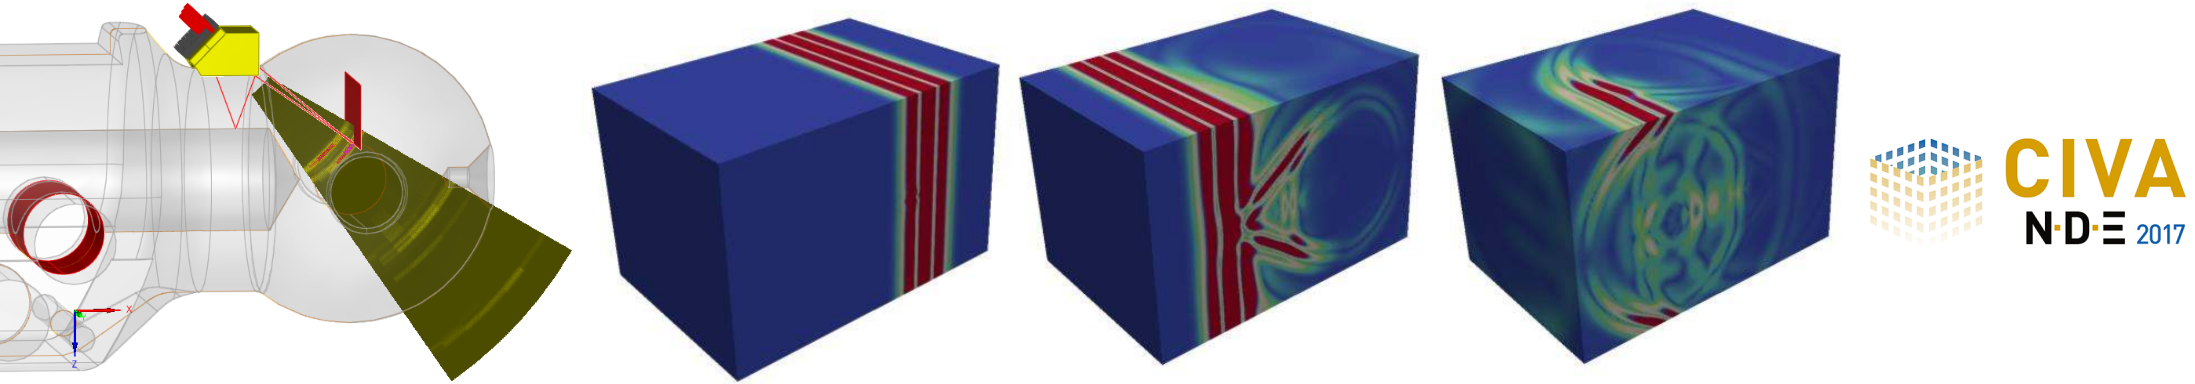
\includegraphics[width=\textwidth]{civa_img_new}%civa_img
%\captionof{figure}{Given a triangular mesh}
%\label{fig:figure1}
\end{minipage}
\footnotesize
 $~^*$ \textcolor{lightblue}{[Imperiale et al. 2019]} A. Imperiale et al , \textit{Coupling strategies between asymptotic and numerical models with application to ultrasonic non-destructive testing of surface flaws}, Journal of Theoretical and Computational Acoustics, 2019.
%\end{tcolorbox}
}
%----------------------------------------------------------------------------------------
%	Objective
%----------------------------------------------------------------------------------------
%\headerbox{Objective}{name=objective,column=0,row=0,span=2,below=context}{
%%%%%%%%%%%%%%%%%%%%%%%%%%%%%%%%%%%%%%%%%%%%%%%%%%%%%%%%%%%%%%%%%%%%%
\headerbox{Pipeline}{name=pipeline,column=0,row=0,span=2,below=context}{
\vspace{-0.15cm}
%%%%%%%%%%%%%%%%%%%%%%%%%%%%%%%%%%%%%%%%%%%%%%%%%%%%%%%%%%%%%%%%%%%% 
\noindent
%\begin{comment}
%	\mybox{
%		
%		\begin{enumerate}[label=\fcolorbox{white}{ceagreen}{\arabic*}, font=\color{white} ]
%			\item Given triangular mesh
%			\item Contruct cross-field
%				(solving PDE, or input CF)
%			\item Identify singularities 
%				(discontinuities in the CF)
%			\item Trace separatrices of the CF
%			 \\(partition the mesh into quadrilateral blocks) 
%			 \item Remesh resulted quads
%		\end{enumerate}
%	}
%	\hfill
	%\includegraphics[scale=0.05]{fleche}
%	\hfill

%	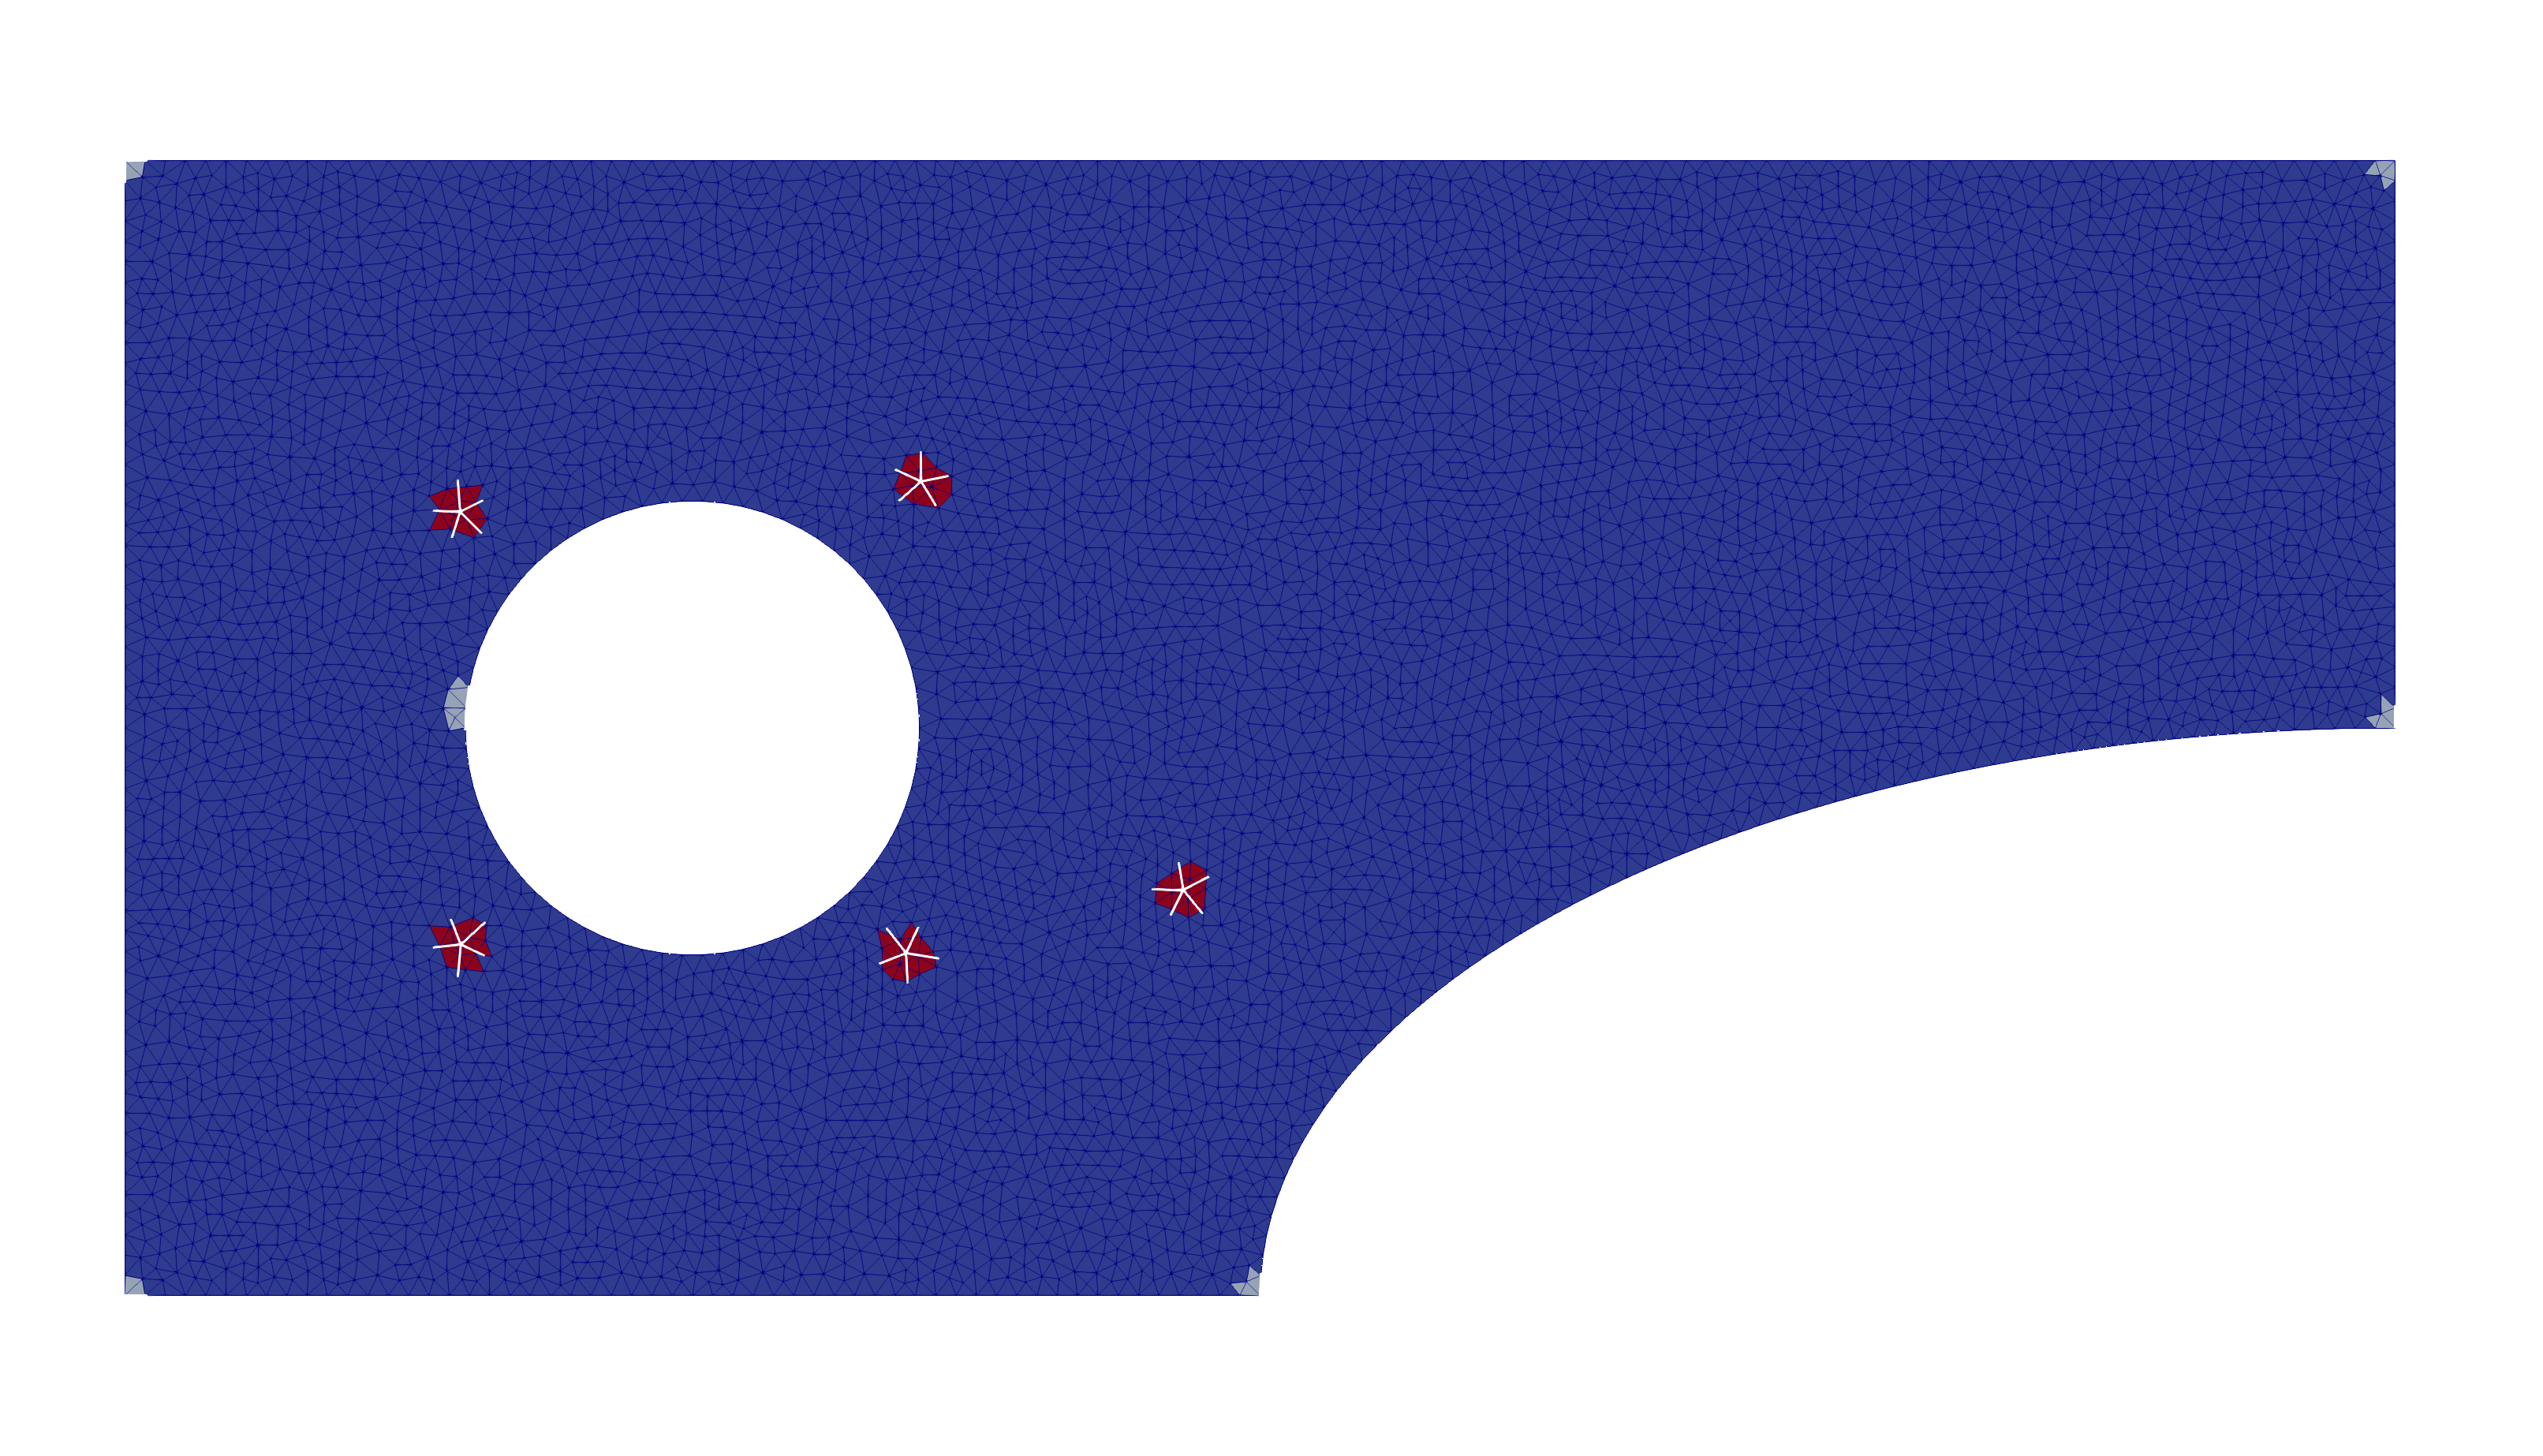
\includegraphics[height=3.7cm]{sing_slots}
%	\captionof{figure}{Simultaneous Strategy}
 %   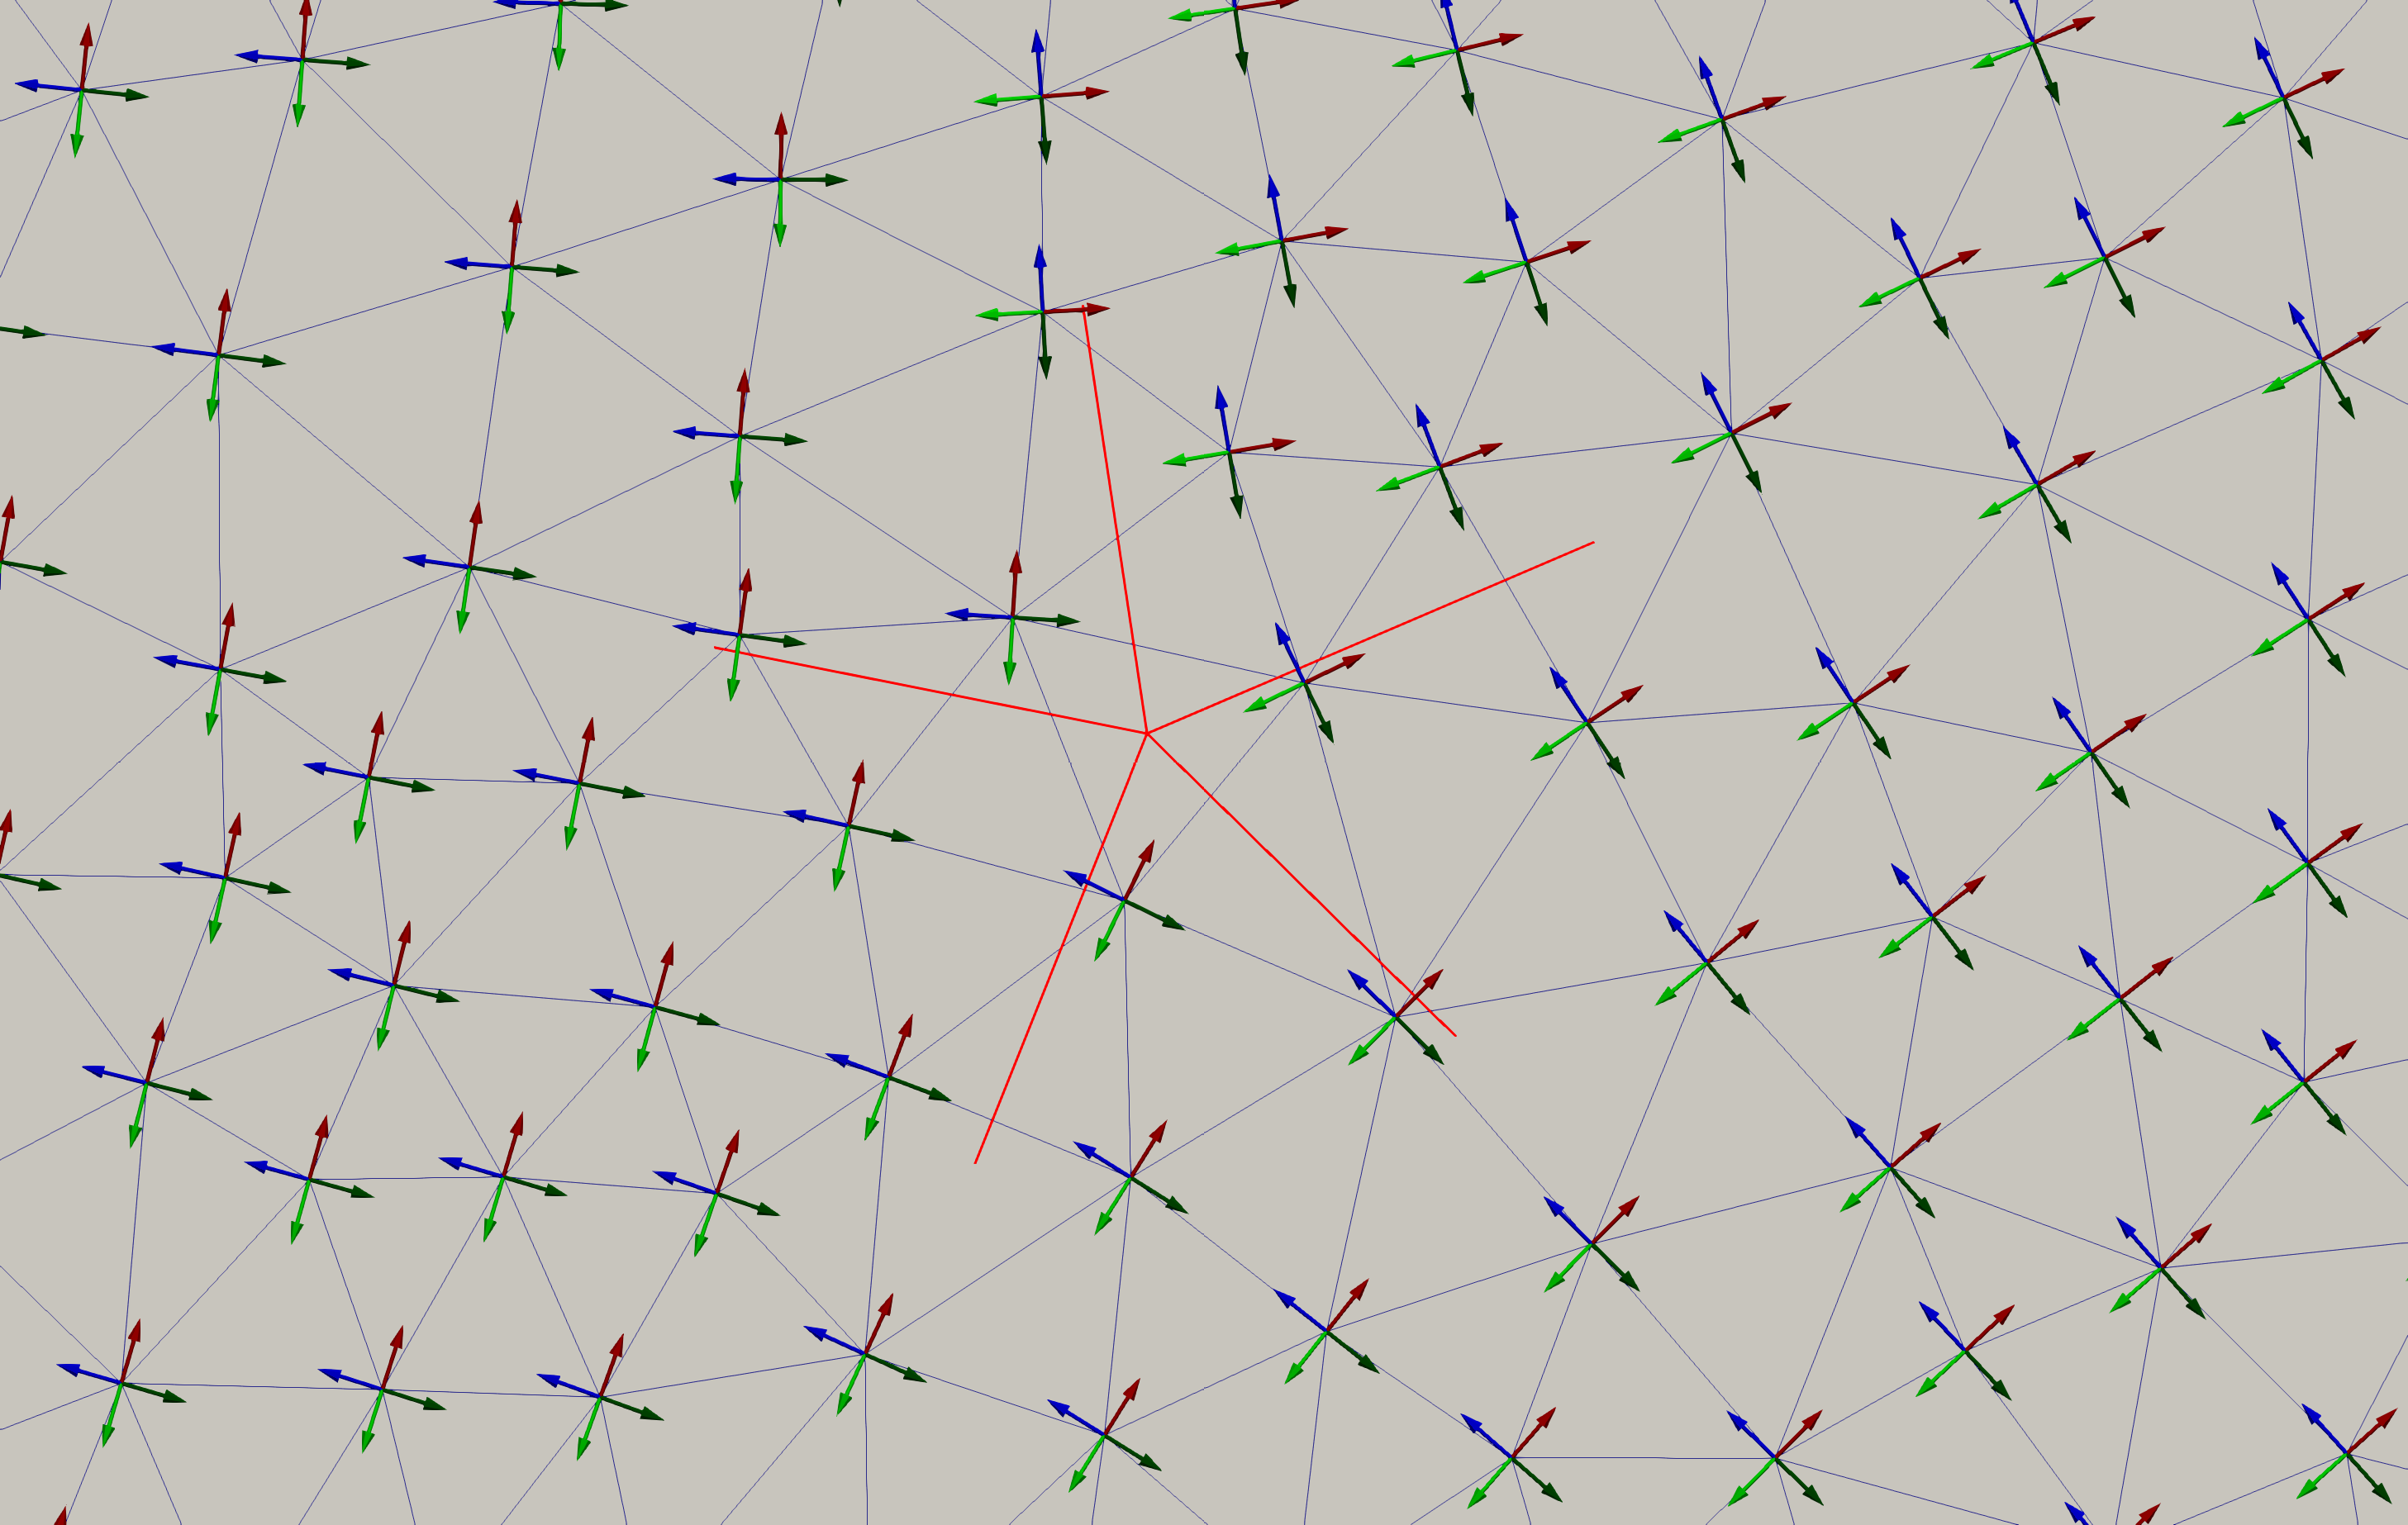
\includegraphics[height=3.7cm]{HIS-Slots-close-up}
  %  \captionof{figure}{Simultaneous Strategy}
   %% 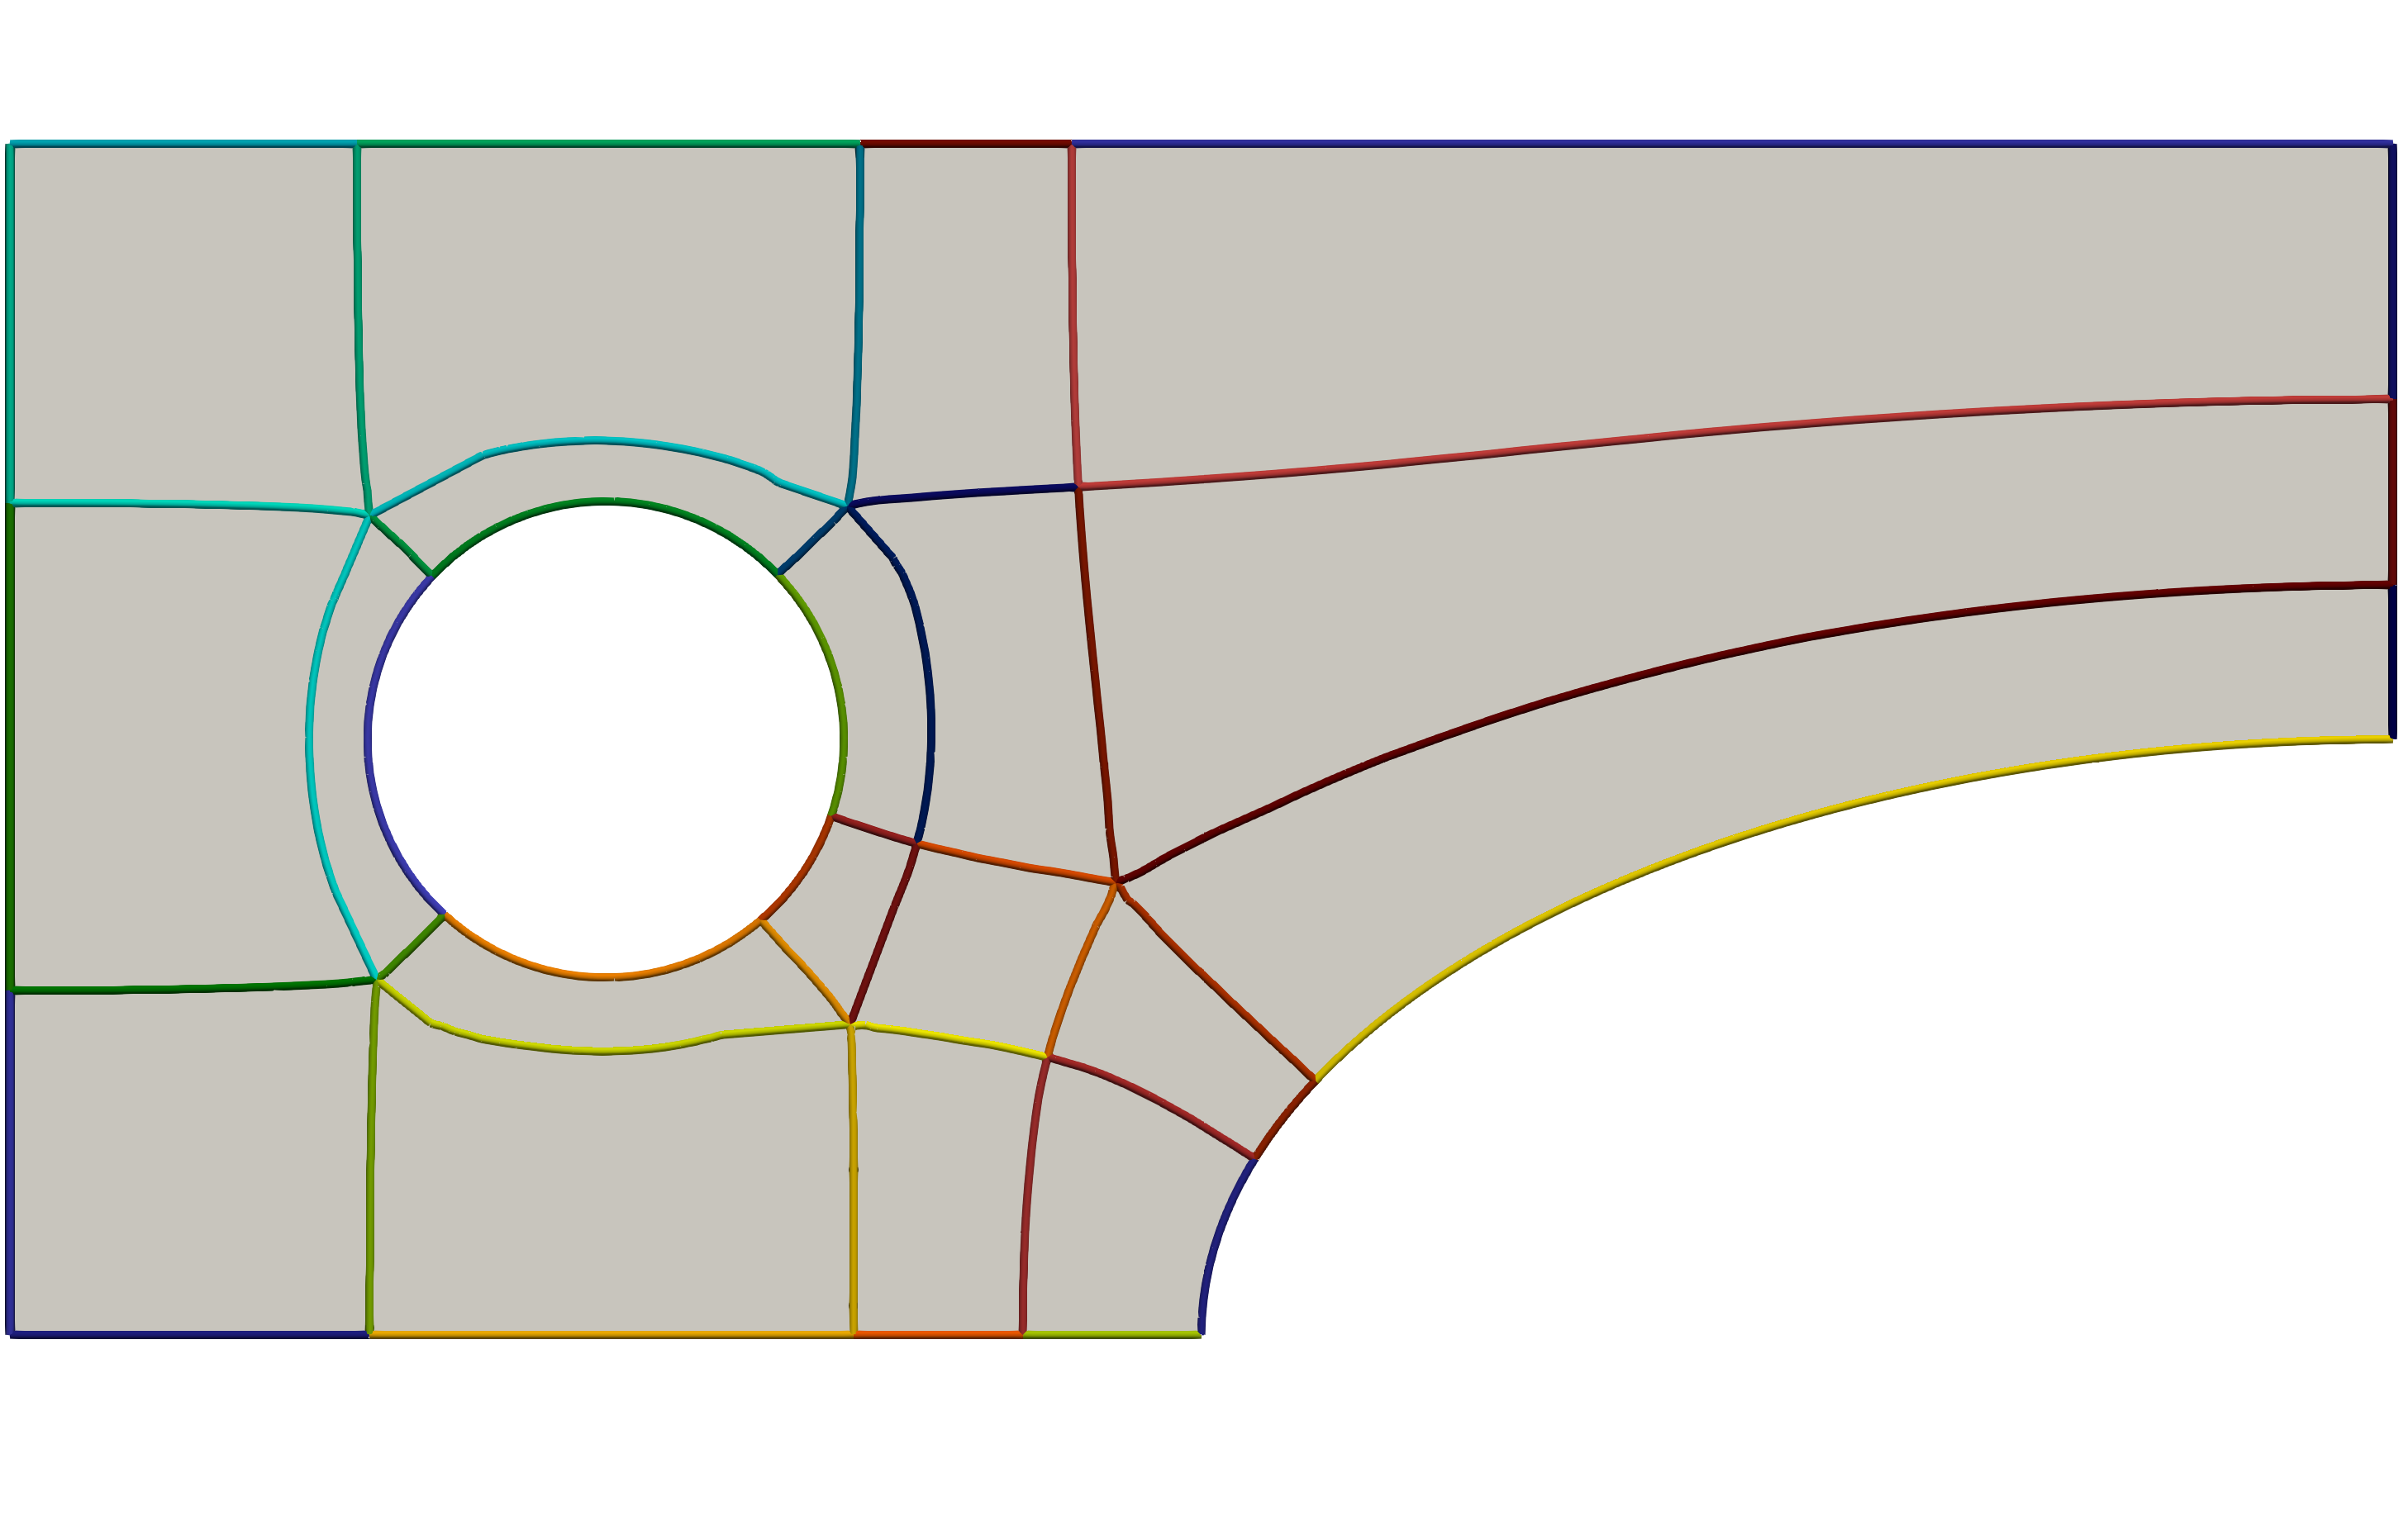
\includegraphics[height=3.7cm]{HIS-SingGraphOriginal-ConfusBallRad005}
  %  \captionof{figure}{Simultaneous Strategy}
  %  \hfill
%\includegraphics[scale=0.05]{fleche}
%\hfill
%\end{comment}
\captionsetup{width=0.13\linewidth}
   % 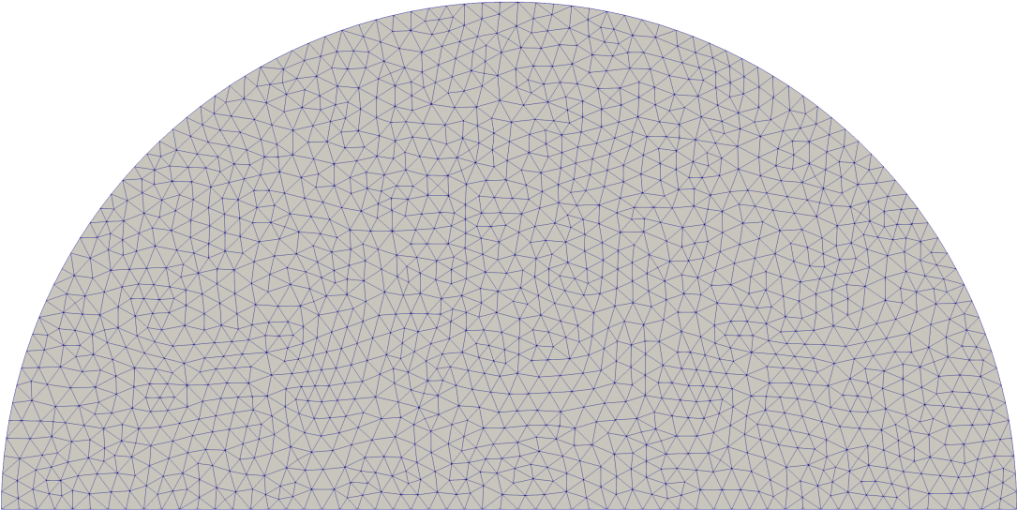
\includegraphics[width=0.2\linewidth]{1}
    %\captionof{figure}{Caption A}
\captionsetup{labelformat=empty}
\noindent
\begin{minipage}[b]{0.13\linewidth}
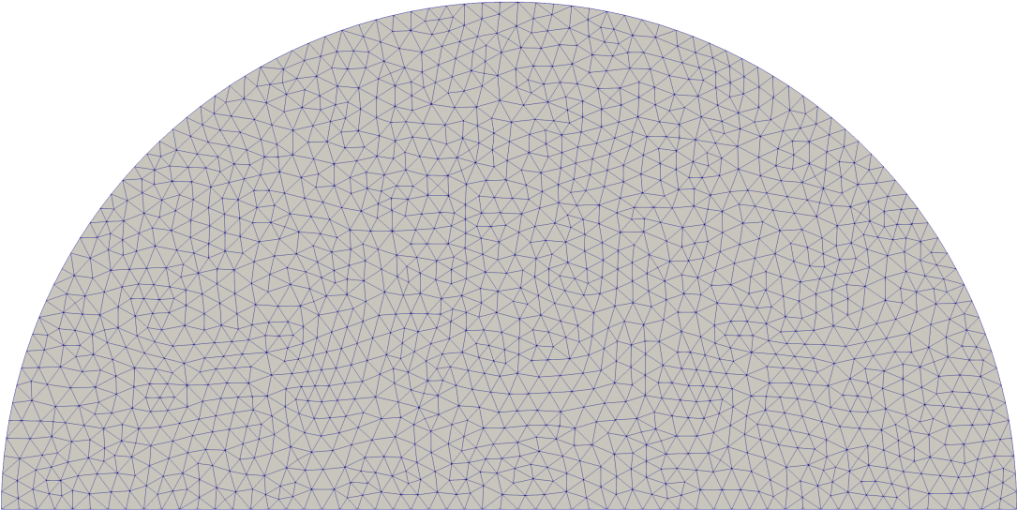
\includegraphics[width=0.99\linewidth]{1}
\captionof{figure}{Triangular mesh}
\label{fig:figure1}
\end{minipage}
\begin{minipage}[b]{0.13\linewidth}
%\hspace{0.001\linewidth}
%\begin{minipage}[b]{0.235\linewidth}
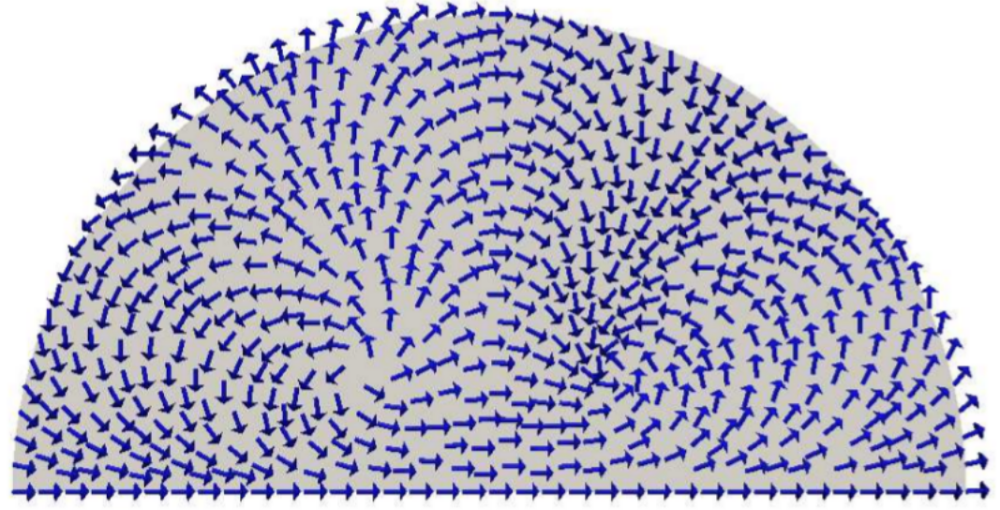
\includegraphics[width=0.99\linewidth]{2}
\captionof{figure}{Cross-Field (CF)}
\label{fig:figure2}
\end{minipage}
%-------------------------------------------------------------------------------------
\begin{minipage}[b]{0.13\linewidth}
%\begin{minipage}[b]{0.235\linewidth}
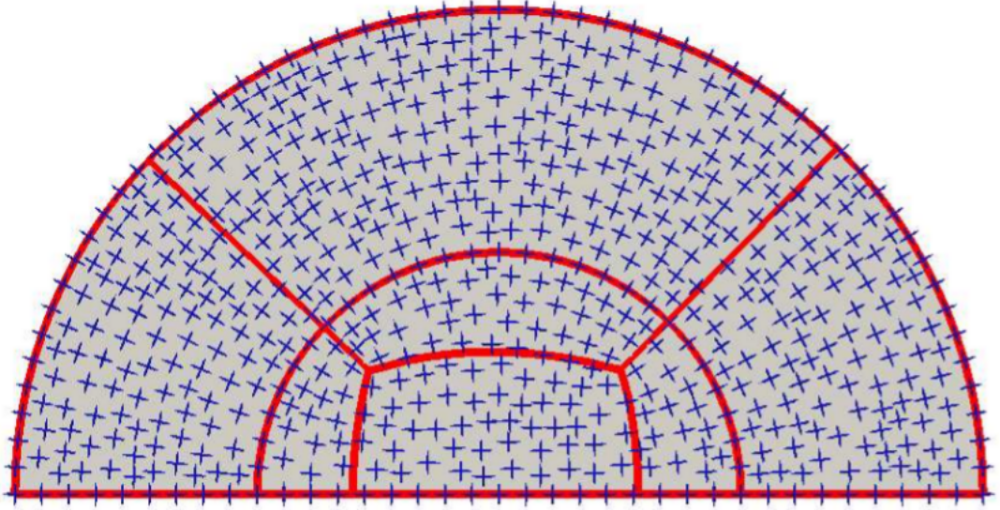
\includegraphics[width=0.99\linewidth]{3}
\captionof{figure}{\textcolor{red}{\textbf{Singularity Graph}}}
\label{fig:figure3}
\end{minipage}
%------------------------------------------------------------------------------------------------
\begin{minipage}[b]{0.13\linewidth}
%\hspace{0.001\linewidth}
%\begin{minipage}[b]{0.235\linewidth}
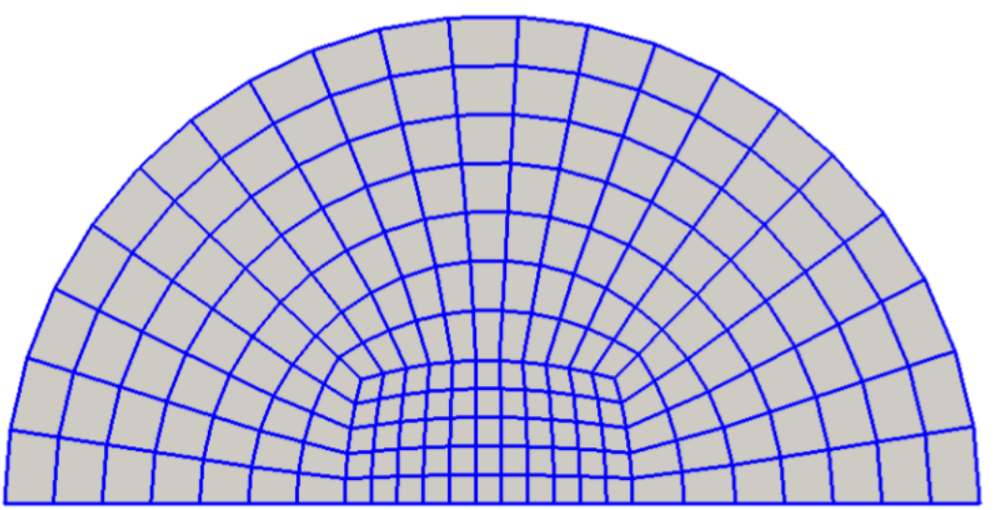
\includegraphics[width=0.99\linewidth]{4}
\captionof{figure}{Resulted quads}
\label{fig:figure4}
\end{minipage}
\begin{minipage}[b]{0.46\linewidth}
The automation of the cross-field generation from a GMSH geometry.

Study and propose a robust block extraction method. 

Work and improve on: \footnotesize \textcolor{lightblue}{[Kowalski et al. 2014]} N. Kowalski, F. Ledoux, and P. Frey, \textit{Automatic domain partitioning for quadrilateral meshing with line constraints}, Engineering with Computers, December 2014.
%\bigskip
%\begin{minipage}[b]{0.99\linewidth}
%includegraphics[width=\textwidth]{Heun}
%\captionof{figure}{llustration of the integration process over a triangle}
%\label{fig:figure2}
\end{minipage}
%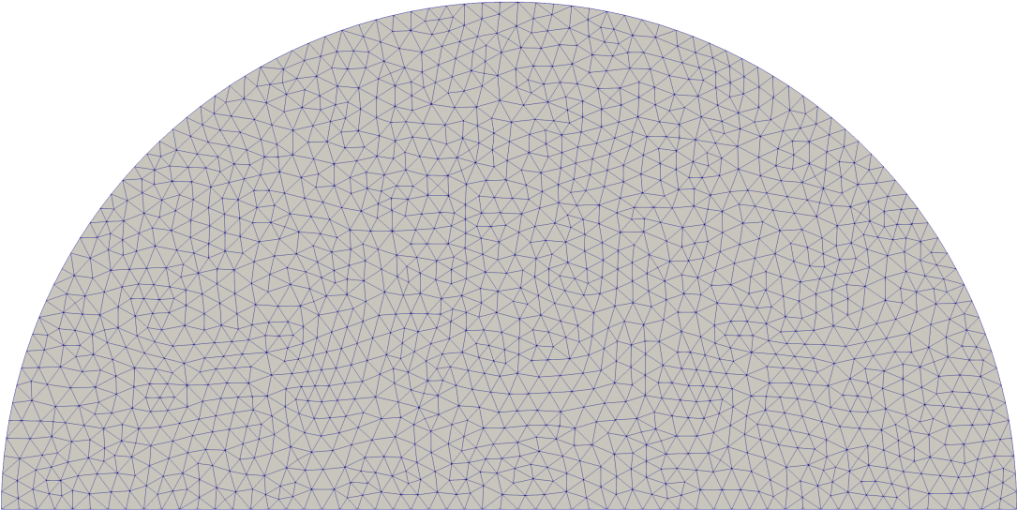
\includegraphics[height=3cm]{1}
%\captionof{figure}{Given triangular mesh}
%          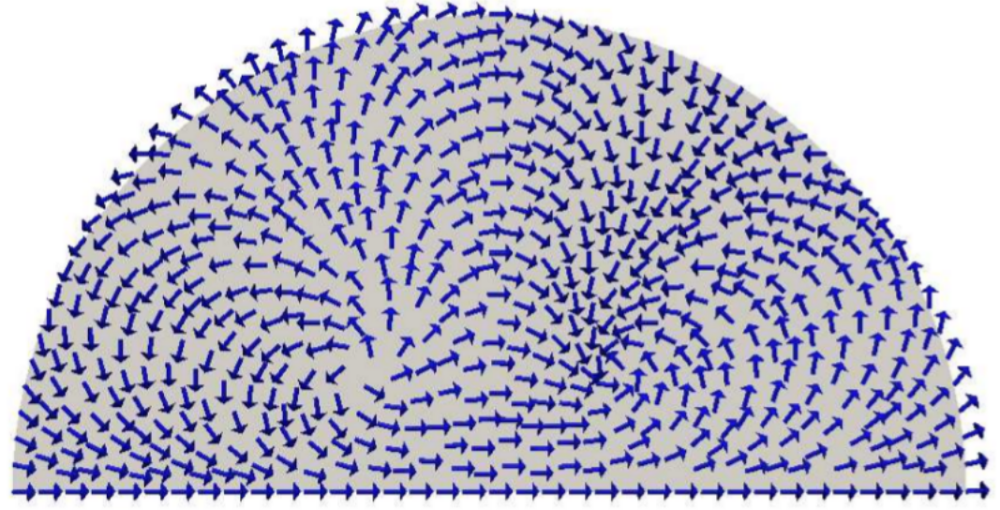
\includegraphics[height=3cm]{2}
%         \captionof{figure}{Contruct cross-field}
%          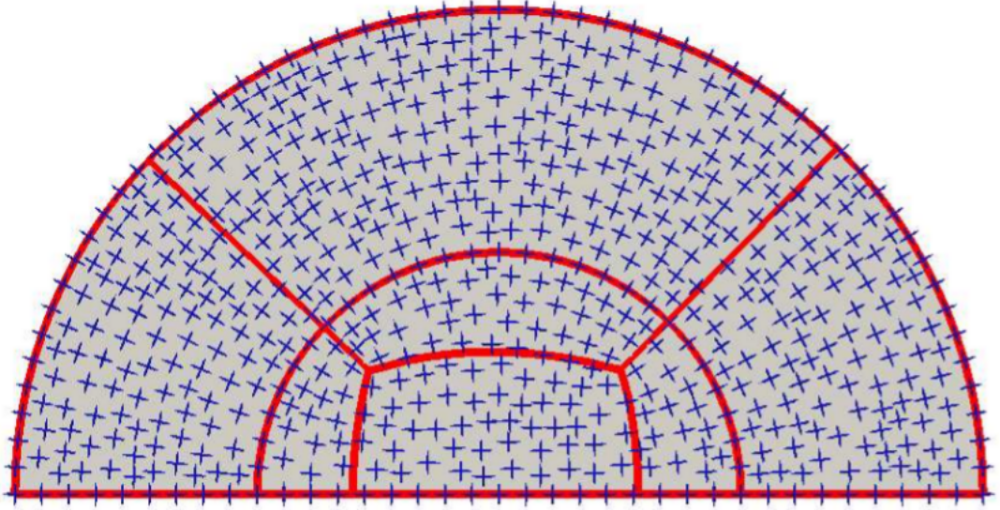
\includegraphics[height=3cm]{3}
%         \captionof{figure}{Trace separatrices of the CF}
%         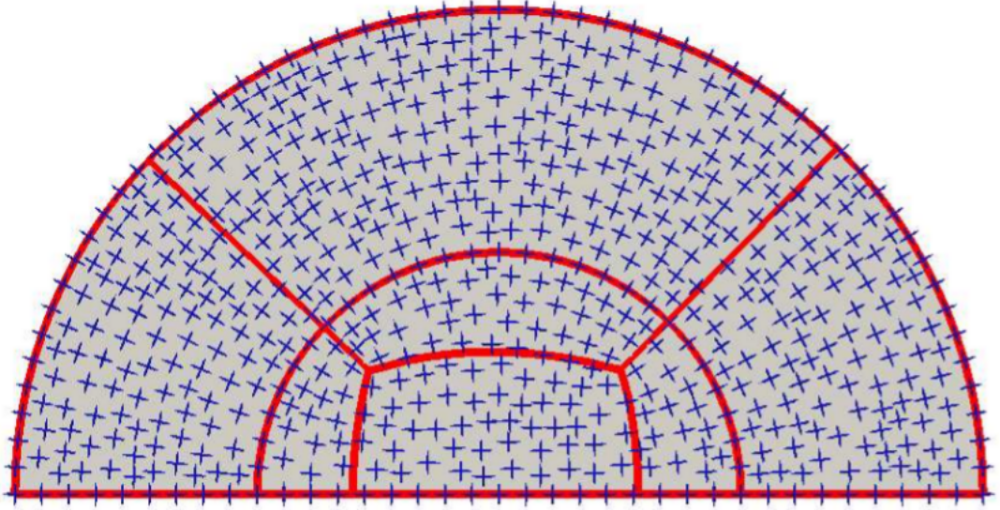
\includegraphics[height=3cm]{3}
%         \captionof{figure}{Remesh resulted quads}
}
%----------------------------------------------------------------------------------------
%	Approach
%----------------------------------------------------------------------------------------
%%%%%%%%%%%%%%%%%%%%%%%%%%%%%%%%%%%%%%%%%%%%%%%%%%%%%%%%%%%%%%%%%%%%%
\headerbox{Singularity Graph Extraction}{name=approach,column=0,row=0,below=pipeline}{
%%%%%%%%%%%%%%%%%%%%%%%%%%%%%%%%%%%%%%%%%%%%%%%%%%%%%%%%%%%%%%%%%%%%%
\noindent
\begin{minipage}[b]{1\linewidth}
\vspace{-0.1cm}\noindent
\begin{tcolorbox}[colframe=gray,boxrule=0.01pt,left=0mm,right=0mm,title=\Large $\ \ \ \ \ \ \ \ \ \ \ \ \ \ \ \ \ $Objectives $\ \ \ \ \ \ \ \ \ \ \ \ \ \ \ \ \ \ \ \ $Limitations$\ \ \ \ \ \ \ \ \ \ \ \ \ \ \ \ \ $]		%\begin{itemize}
\vspace{-0.2cm}\noindent
$\bullet$ Fully automatic method  $\ \ \ \ \ \ \ \ \ \ \ \ \ \bullet$  Dependence on input triangulation%	\item[$\bullet$] Fully automatic method
\newline
$\bullet$ High quality resulted quad blocks $\ \ \ \ \ \ \bullet$ Approximation errors%	\item[$\bullet$] High quality resulted quad blocks
\vspace{-0.2cm}
\end{tcolorbox}
\vspace{-0.2cm}
Difficulty  to achieve robustness for quad-block decomposition.
\end{minipage}
\vspace{-1cm}
}
%----------------------------------------------------------------------------------------
%	Implementation
%----------------------------------------------------------------------------------------
%%%%%%%%%%%%%%%%%%%%%%%%%%%%%%%%%%%%%%%%%%%%%%%%%%%%%%%%%%%%%%%%%%%%%
\headerbox{Strategies}{name=strategies,column=0,below=approach}{
\noindent
%%%%%%%%%%%%%%%%%%%%%%%%%%%%%%%%%%%%%%%%%%%%%%%%%%%%%%%%%%%%%%%%%%%%%
\begin{minipage}[b]{1\linewidth}
\vspace{-0.1cm}\noindent
\begin{tcolorbox}[colframe=gray,boxrule=0.01pt,left=0mm,right=0mm,title=\Large Continuous Strategies]
\vspace{-0.2cm}\noindent
(Iteratively/ Simultaneuously) Depart from each singular point along each
slot direction until reaching: \textbf{Iterative} $\rightarrow$ the vicinity of a different singularity (confusing ball), \textbf{Simultaneuous} $\rightarrow$ the vicinity of a different singularity line (thresholdDistance) or the boundary.	
\vspace{-0.2cm}
\end{tcolorbox}
\vspace{-0.1cm}
\end{minipage}
\captionsetup{labelformat=empty}
\noindent
%\begin{minipage}[b]{0.49\linewidth}
%\includegraphics[width=\textwidth]{HIS4-orig-Rad003}
%\captionof{figure}{Sequential Strategy}
%\label{fig:figure5}
%\end{minipage}
%\hspace{0.005\linewidth}
%\begin{minipage}[b]{0.49\linewidth}
%\includegraphics[width=\textwidth]{HIS4-sim-Rad003}
%\captionof{figure}{Simultaneous Strategy}
%\label{fig:figure6}
%\end{minipage}
%	\begin{minipage}[!Ht]{0.49\linewidth}
%	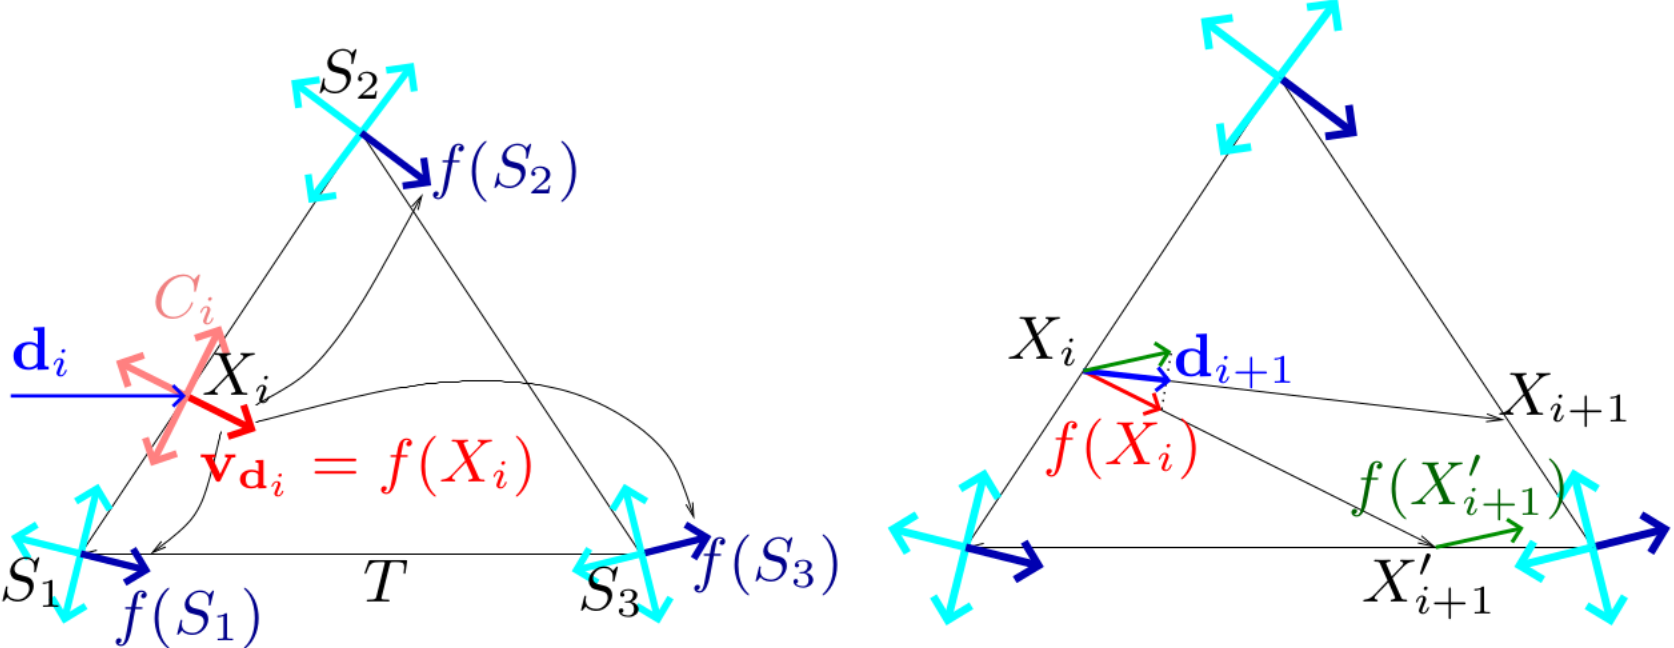
\includegraphics[width=\textwidth]{Heun}
%	\captionof{figure}{Illustration of the integration process (Heun) over a triangle}
%	\label{fig:figure7}
%	\end{minipage}
%	\hspace{0.005\linewidth}
%	\begin{minipage}[!Ht]{0.49\linewidth}
%	\includegraphics[width=\textwidth]{SingZoom}
%	\captionof{figure}{Singularities and slots (left - degree 3, right - degree 5)}
%	\label{fig:figure8}
%	\end{minipage}

%\newline	
\noindent
\begin{minipage}[!HT]{0.5\linewidth}
 \textbf{Challenges}
\newline	
\medskip
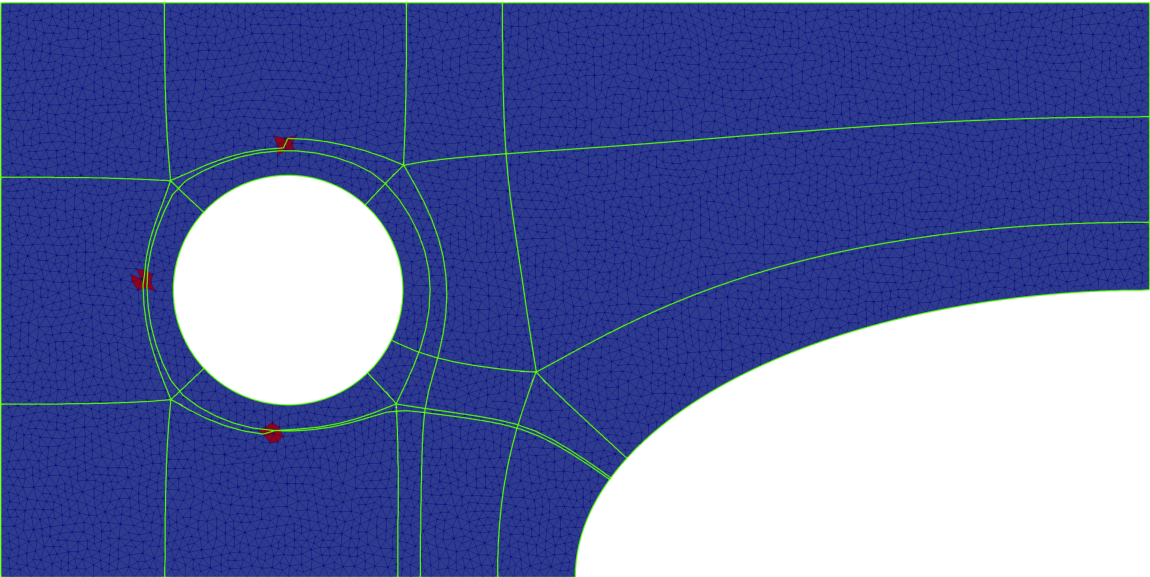
\includegraphics[width=\textwidth]{HIS4-sim-Rad002}
\captionof{figure}{ a) "miss the connection"}
\label{fig:figure9}
\smallskip
\small b) dependence on proximity parameter - confusing ball radius, thresholdDistance
\end{minipage}
\hspace{0.1\linewidth}
%\vspace{0.2cm} 
 \begin{minipage}[!HT]{0.38\linewidth}
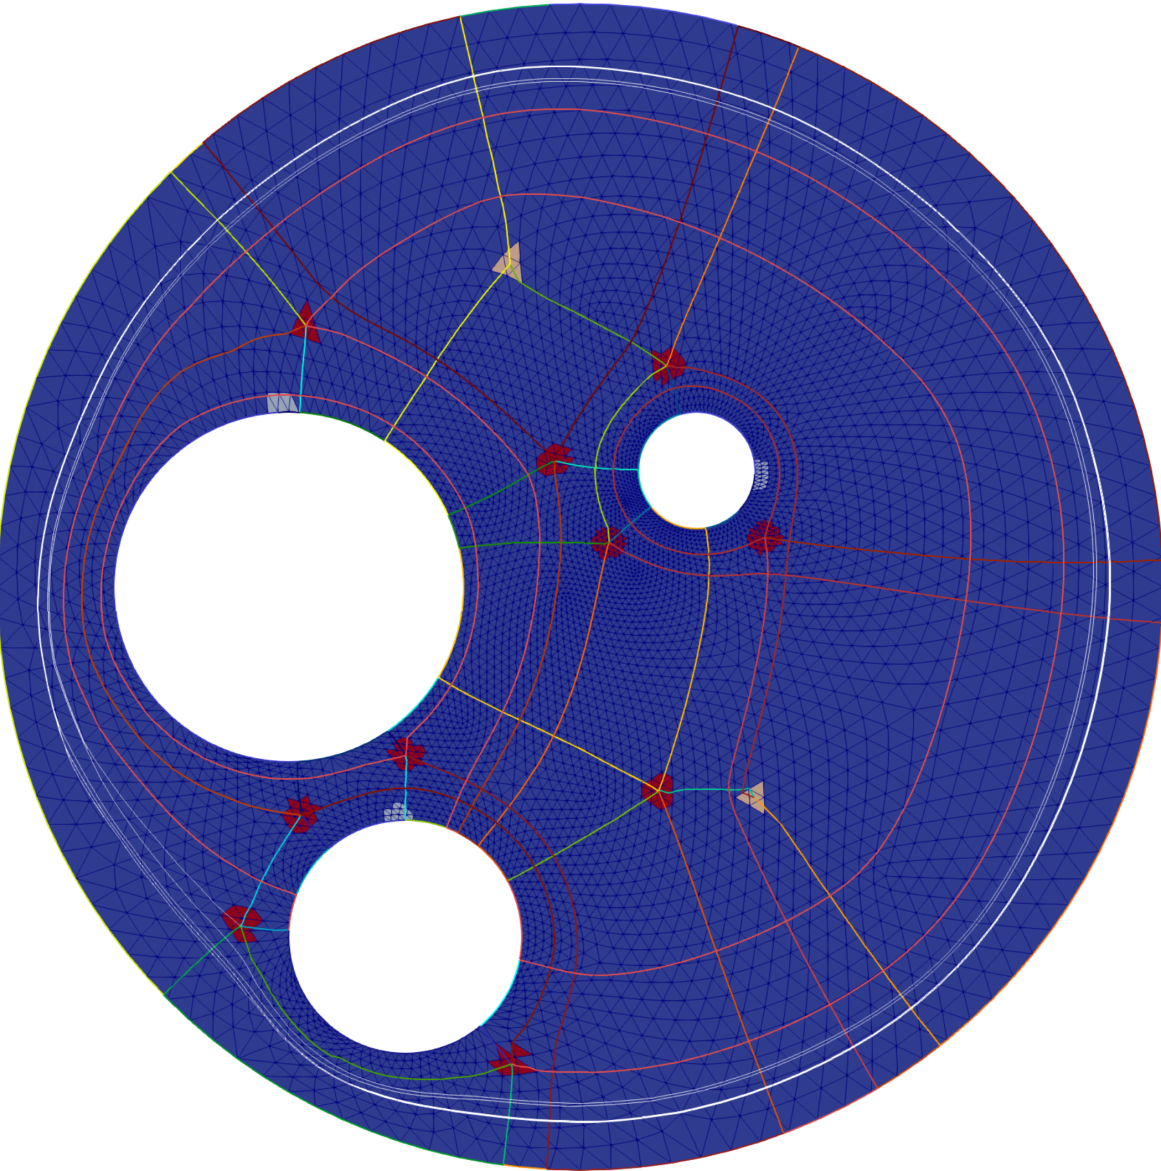
\includegraphics[width=\textwidth]{Circle_with_circle_holes_refSS1-cycle}
\captionof{figure}{ c) Cycles}
\label{fig:figure10}
\end{minipage}
\begin{tcolorbox}[colframe=gray,boxrule=0.01pt,left=0mm,right=0mm,title=\Large Discrete Strategy]
\vspace{-0.2cm} \noindent
Build a Slot Connectivity Graph - modified Dijkstra's algorithm.
\newline
Extract the Singularity Graph - Integer Linear Programming.%minimum weight perfect matching problem with conflict pair constraints (MWPMPC).
\vspace{0.1cm}
\newline
\begin{minipage}[t]{0.5\linewidth}%\begin{flushleft}
\textbf{Advantages}
\newline
\medskip
\noindent
$\bullet$ All possible connections $\rightarrow$ choice
\vspace{-0.2cm}
\newline
$\bullet$ No infinite cycles
\end{minipage}
\begin{minipage}[t]{0.49\linewidth}	%\begin{flushright}
\textbf{Limitations}
\newline
\medskip
$\bullet$ Depends on the mesh resolution
\vspace{-0.2cm}
\newline
$\bullet$ Computationally expensive
\newline
\end{minipage}
\vspace{-0.6cm}
\end{tcolorbox}
\vspace{-0.05cm}
%%%%%%%%%%%%%%%%%
\captionsetup{width=0.35\linewidth}
\captionsetup{labelformat=empty}
\hspace{0.05\linewidth}
\begin{minipage}[b]{0.35\linewidth}
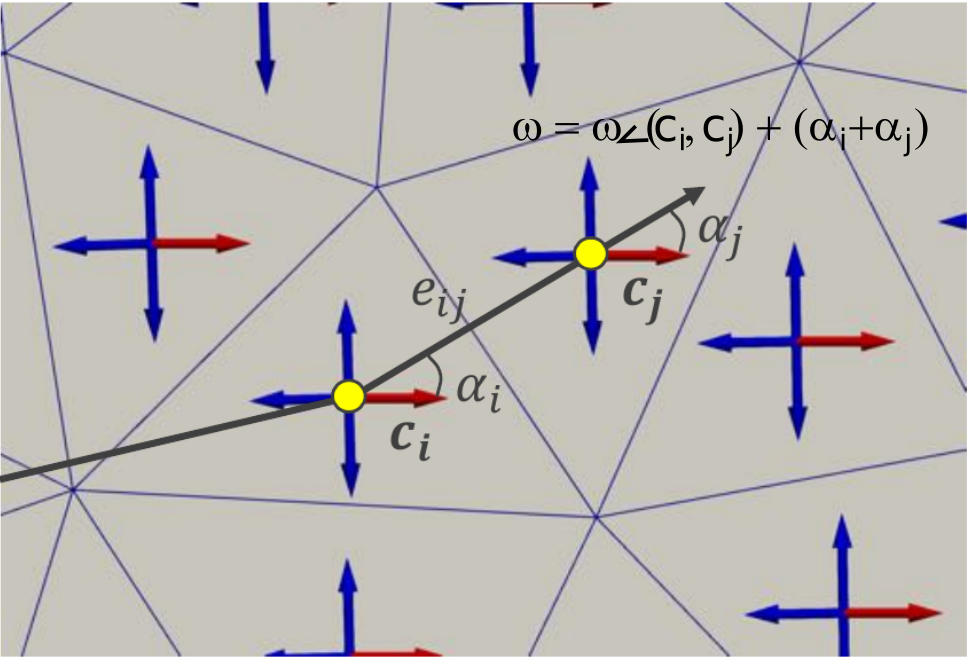
\includegraphics[width=0.99\linewidth]{img4_text}
\captionof{figure}{Edge weight}
\end{minipage}
\hspace{0.09\linewidth}
\begin{minipage}[b]{0.35\linewidth}
%\hspace{0.001\linewidth}
%\begin{minipage}[b]{0.235\linewidth}
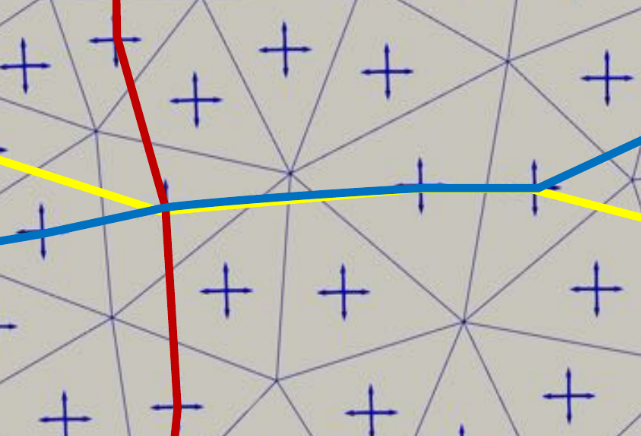
\includegraphics[width=0.99\linewidth]{incomp_edges}
\captionof{figure}{Incompatible edges}
\end{minipage}
%%%%%%%%%%%%%%%%%%%%%%%%%%
%\begin{minipage}[b]{0.49\linewidth}
%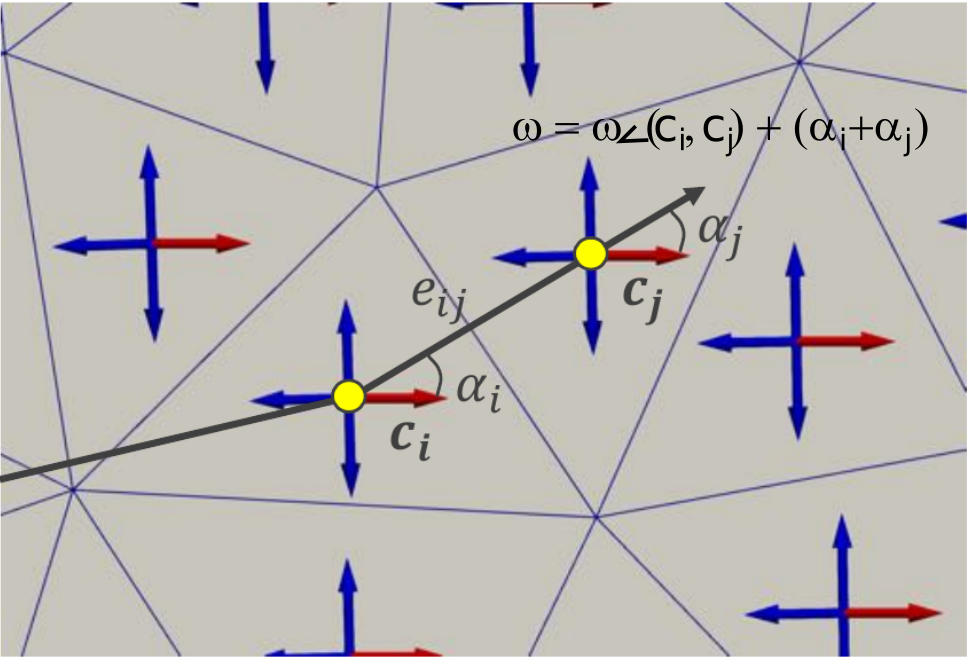
\includegraphics[width=0.49\textwidth]{img4_text}
%\captionof{figure}{Edge weight}
%\end{minipage}
%\hspace{0.005\linewidth}
%\begin{minipage}[b]{0.49\linewidth}
%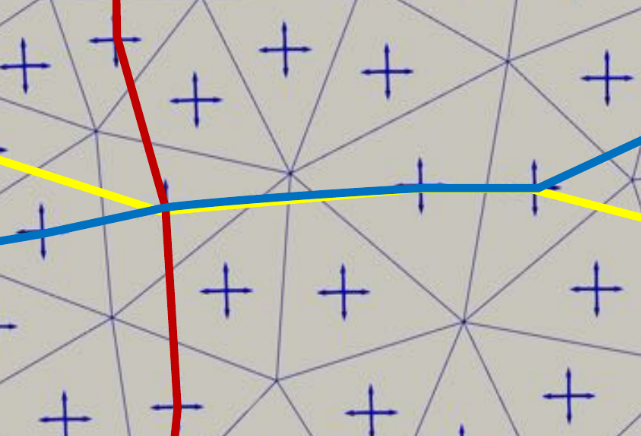
\includegraphics[width=0.49\textwidth]{incomp_edges}
%\captionof{figure}{Incompatible edges}
%\end{minipage}
%%%%%%%%%%%%%%%%%%%	
%
%\begin{minipage}[b]{0.5\linewidth}%\begin{flushleft}
%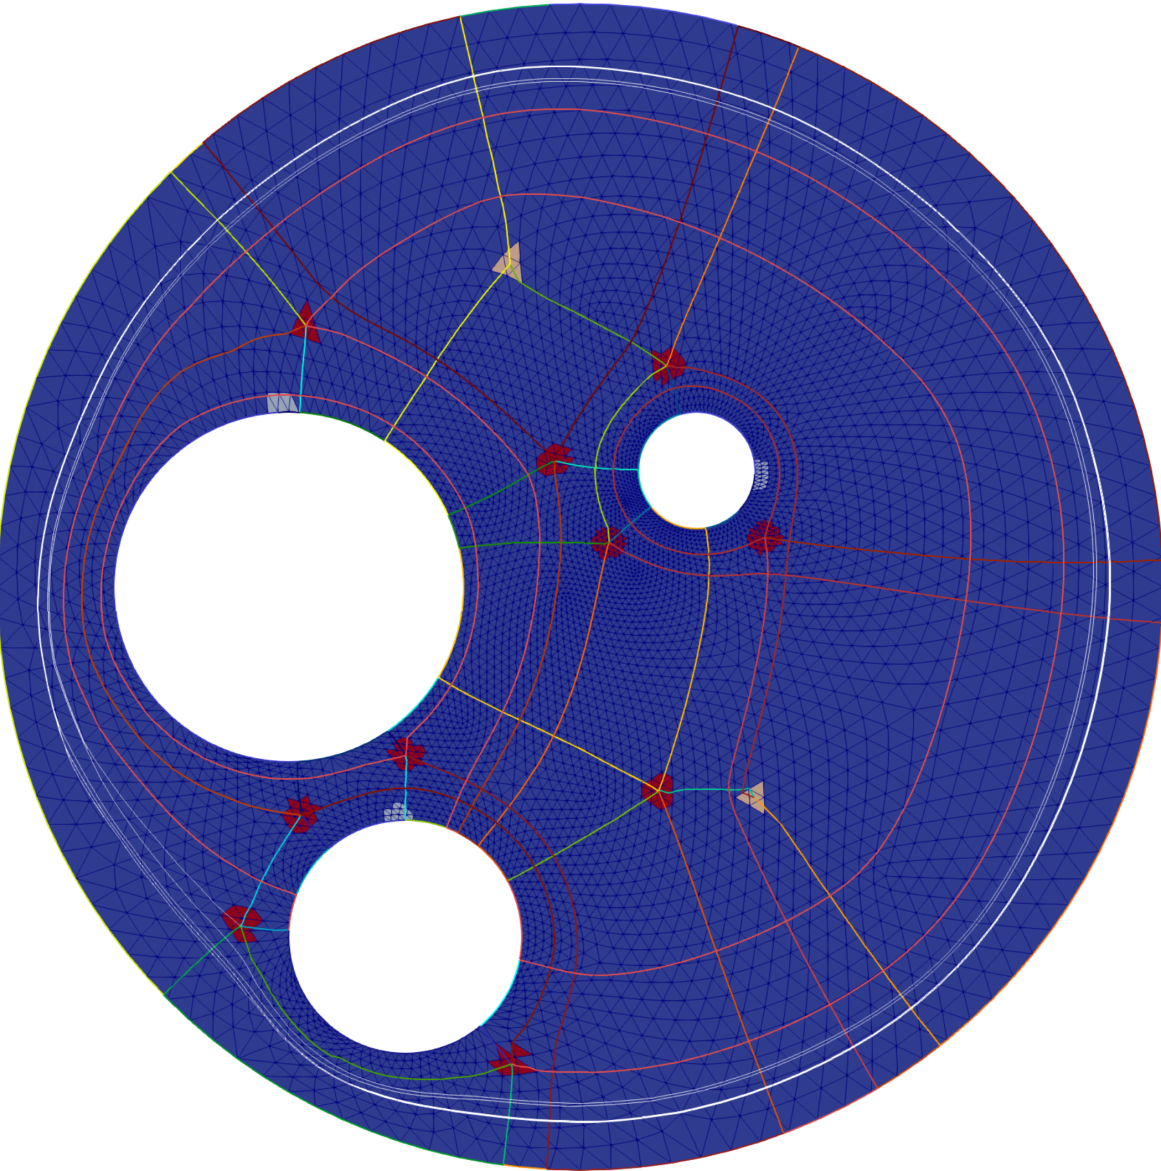
\includegraphics[width=\textwidth]{Circle_with_circle_holes_refSS1-cycle}
%\captionof{figure}{ a) Cycles}
%\label{fig:figure2}%\end{flushleft}
%\end{minipage}
%\begin{minipage}[b]{0.49\linewidth}%\begin{flushright}
%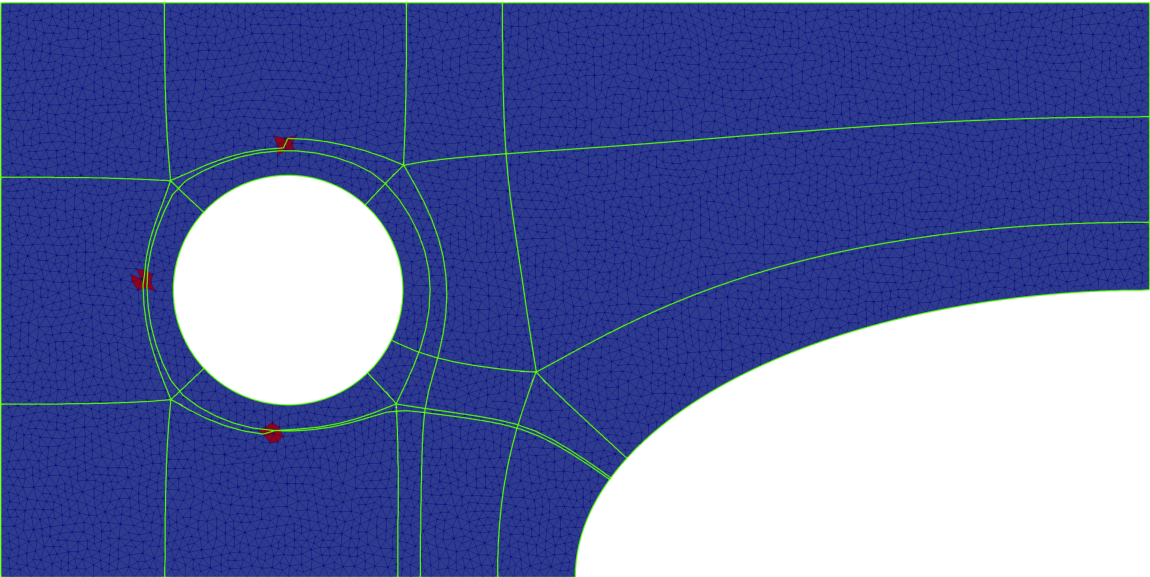
\includegraphics[width=\textwidth]{HIS4-sim-Rad002}
%\captionof{figure}{ b) "miss the connection"}
%\label{fig:figure2}
%	\bigskip
%	
%$c)$ dependence on proximity parameter - confusing ball radius, thresholdDistance
%
%%%%\end{flushright}
%\end{minipage}
%\bigskip
}
%--------------------------------------------------------------------------------------------
%\headerbox{}%
%{name=foottext, column=0, above=bottom, textborder=none, headerborder=none, boxheaderheight=0pt}
  %----------------------------------------------------------------------------------------
%	Experimentation
%----------------------------------------------------------------------------------------
%%%%%%%%%%%%%%%%%%%%%%%%%%%%%%%%%%%%%%%%%%%%%%%%%%%%%%%%%%%%%%%%%%%%%
\headerbox{Discrete Strategy - Results}{name=experimentation,column=1,below=pipeline}{
%%%%%%%%%%%%%%%%%%%%%%%%%%%%%%%%%%%%%%%%%%%%%%%%%%%%%%%%%%%%%%%%%%%%%
\captionsetup{labelformat=empty}
%%%%%%%%%%%%%%%%%%%%%%%%%%%%%%%%%%%%%%%%%%%%%%%%%%%%%%
\noindent
%\begin{minipage}[b]{0.53\linewidth}%\begin{flushleft}
%\vspace{0.57cm}	
%\textbf{Algorithm}
% $\bullet$ Original Mesh: $M = (V, E, T)$
% \newline 
% 
% $\bullet$ Construct Connectivity Graph: 
% \newline
% $\mathcal{G} = (\mathcal{V}, \mathcal{E})$; $\mathcal{V} = centers\{T\}$; 
% $\mathcal{E}(\mathcal{V_i}, \mathcal{V_j}) \Rightarrow T_i \cap T_j \neq \emptyset$
%\newline
%
%$\bullet$ Construct Slot-Connectivity Graph: $\mathcal{G}_{\mathcal{S}} = (\mathcal{V_S}, \mathcal{E_S})$, $\mathcal{V_S} = Singularity-{Slots} + boundary$, 
% \newline
% using Dijkstra - each $\mathcal{E_S}$ - assigned a weight inversely proportional to the "flow alignment"
%  \newline 
% 
% $\bullet$ Construct Singularity Graph:  
% \newline
% Optimization: binary variables - presence of $\mathcal{E_S}$; exactly one $\mathcal{E_S}$ per slot; constrain incompatible edges $\forall (\mathcal{E_S}_i, \mathcal{E_S}_j) \in CI, \mathcal{E_S}_i + \mathcal{E_S}_j \leq 1$  
% \newline
% 
 %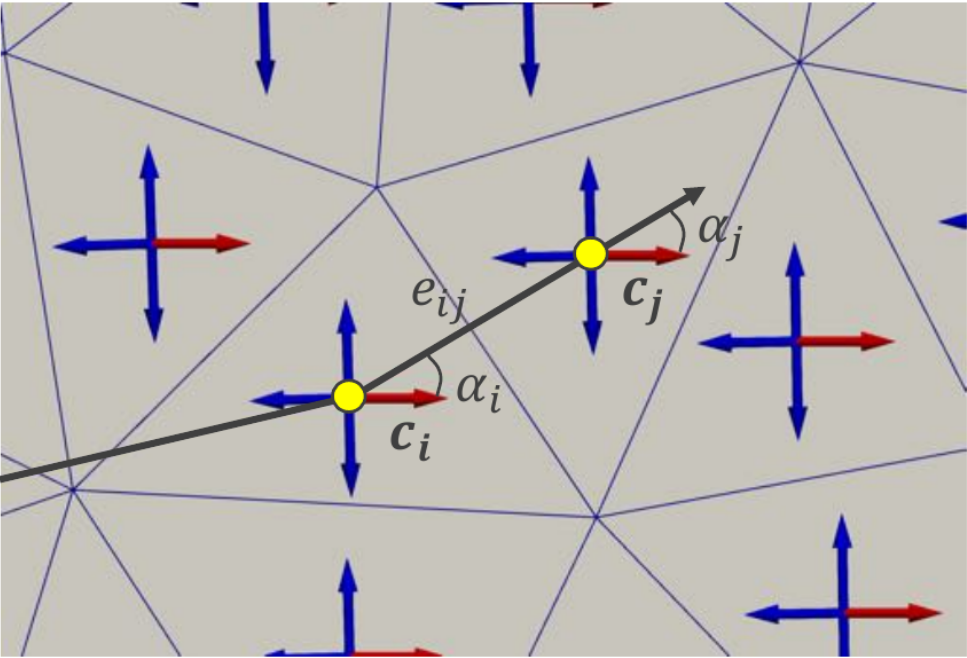
\includegraphics[width=\textwidth]{img3}
%	\begin{algorithmic}[1]
%	\State $dist[source]\gets 0;$
%	\While{$Q\not=\emptyset$}
%	\State $u:= center\ of\ triangle\ in\ Q;$
%	\State $Q\gets Q\setminus u;$
%	\If{$u\in Targets$}
%	\State{$dist[u] = dist[u] + w\_penalty * \angle(CT_{previous}[u] -CT_{target\_slot\_u});$}
%	\State{$return\ u;$}
%	\EndIf
%	\For{$v\in Neigh(u); v\ not\ visited$}
%\State $\widetilde{CT_v}\gets closest\ {CT_v}\ w.r.t\ \widetilde{CT_u};$
%\State $dist_{temp}\gets dist[u] + w\_penalty * \angle(\widetilde{CT_u}, \widetilde{CT_v}) + 	\%angle(\widetilde{CT_v}, \overrightarrow{uv});$
%	\If{$dist_{temp} < dist[v]$}
%	\State $dist[v]\gets dist_{temp};$
%	\State $previous[v] = u;$
%	\State $CT_{previous}[v] = \widetilde{CT_v};$
%	\EndIf
%	\EndFor
%	EndWhile
%\end{algorithmic}
 \noindent
 \vspace{0.41cm}
 \begin{minipage}[b]{0.38\linewidth}%\begin{flushright}
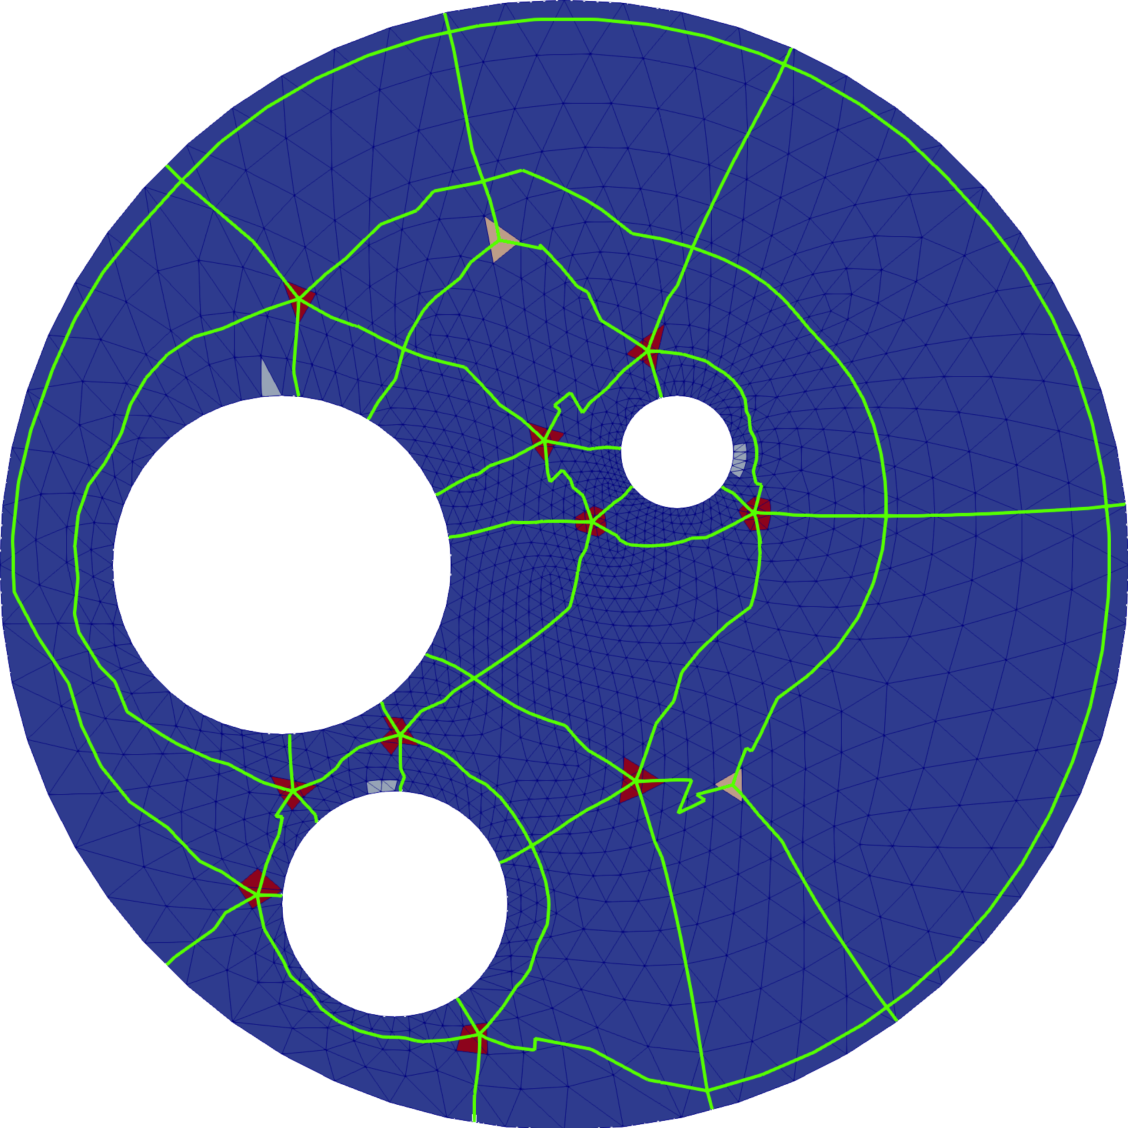
\includegraphics[width=\textwidth]{CWCH_coarse-shortest_paths}%\end{flushleft}
\captionof{figure}{No cycles result} 
\end{minipage}
\begin{minipage}[b]{0.25\linewidth}
%\hspace{0.005\linewidth}
%\vspace{0.2cm}	
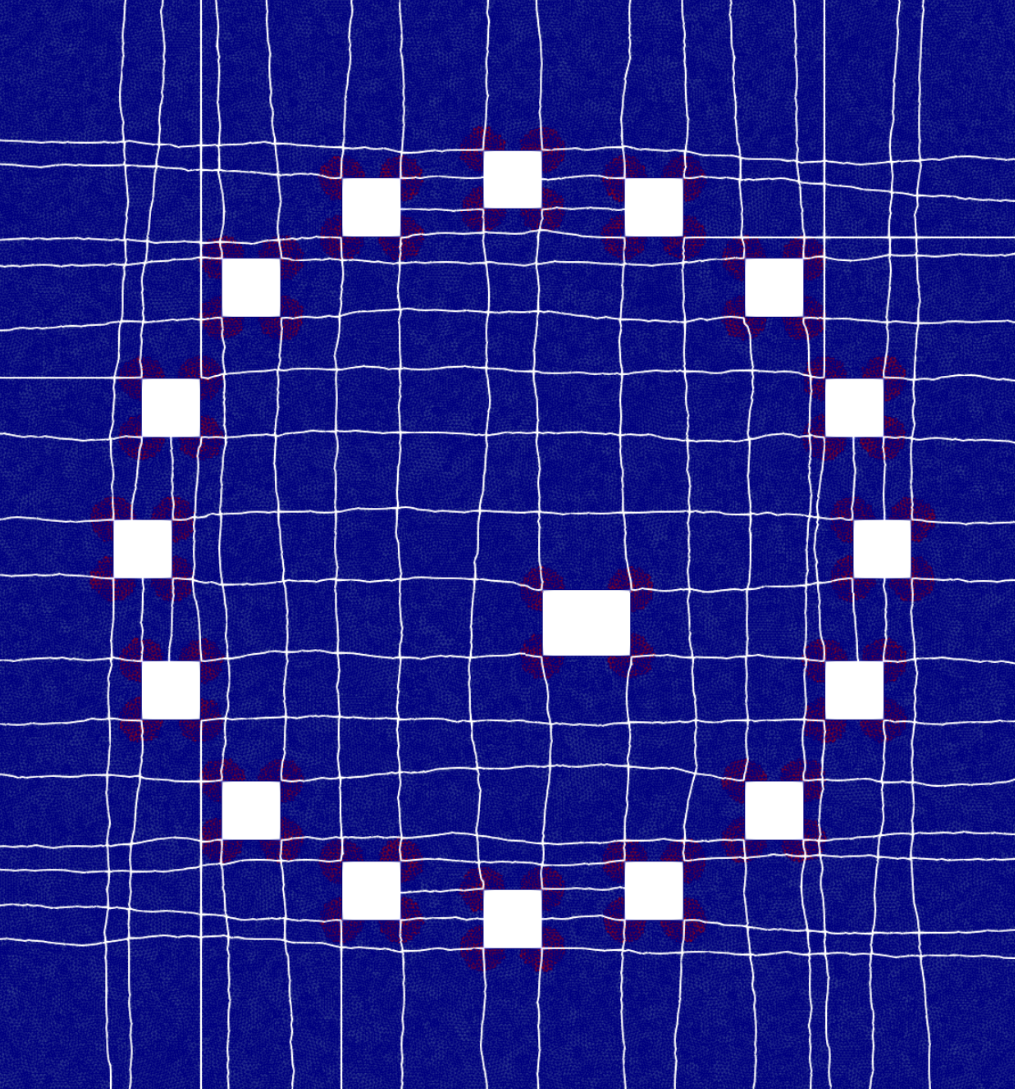
\includegraphics[width=\textwidth]{Tomo}
\captionof{figure}{Geometric slots}
\end{minipage}
%%%%%%%%%%%%%%%%%%%%%%%%%%%%%%%%%
\begin{minipage}[b]{0.35\linewidth}
  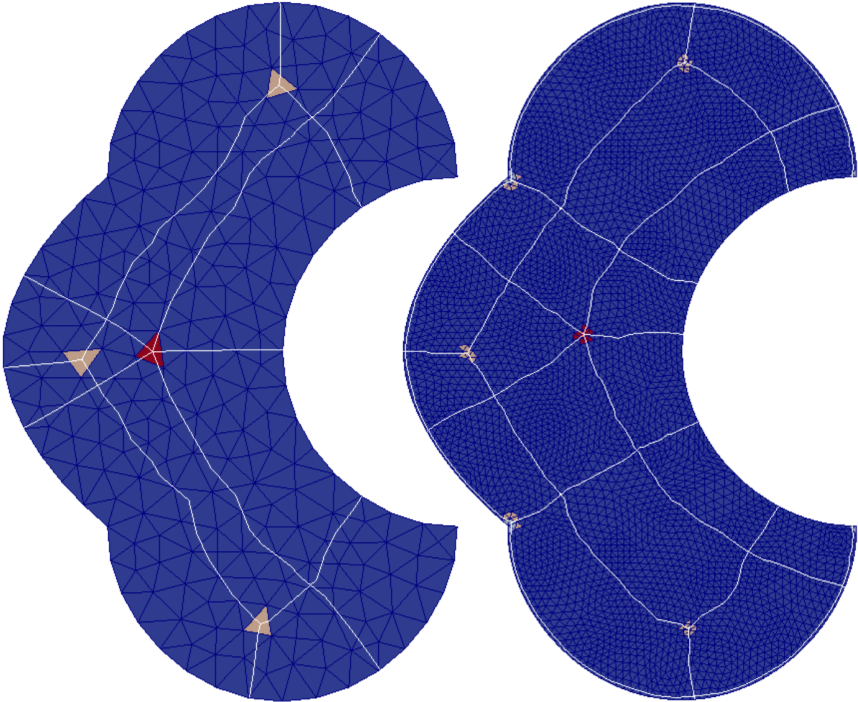
\includegraphics[width=\textwidth]{flower_img}
  \captionof{figure}{Without (left) with (right) geometric slots}
\end{minipage}
\vspace{0.41cm}
%\vspace{0.05\linewidth}
%%%%%%%%%%%%%%%%%%%%%%%%%%%%%%%%%
\begin{minipage}[b]{0.48\linewidth}
  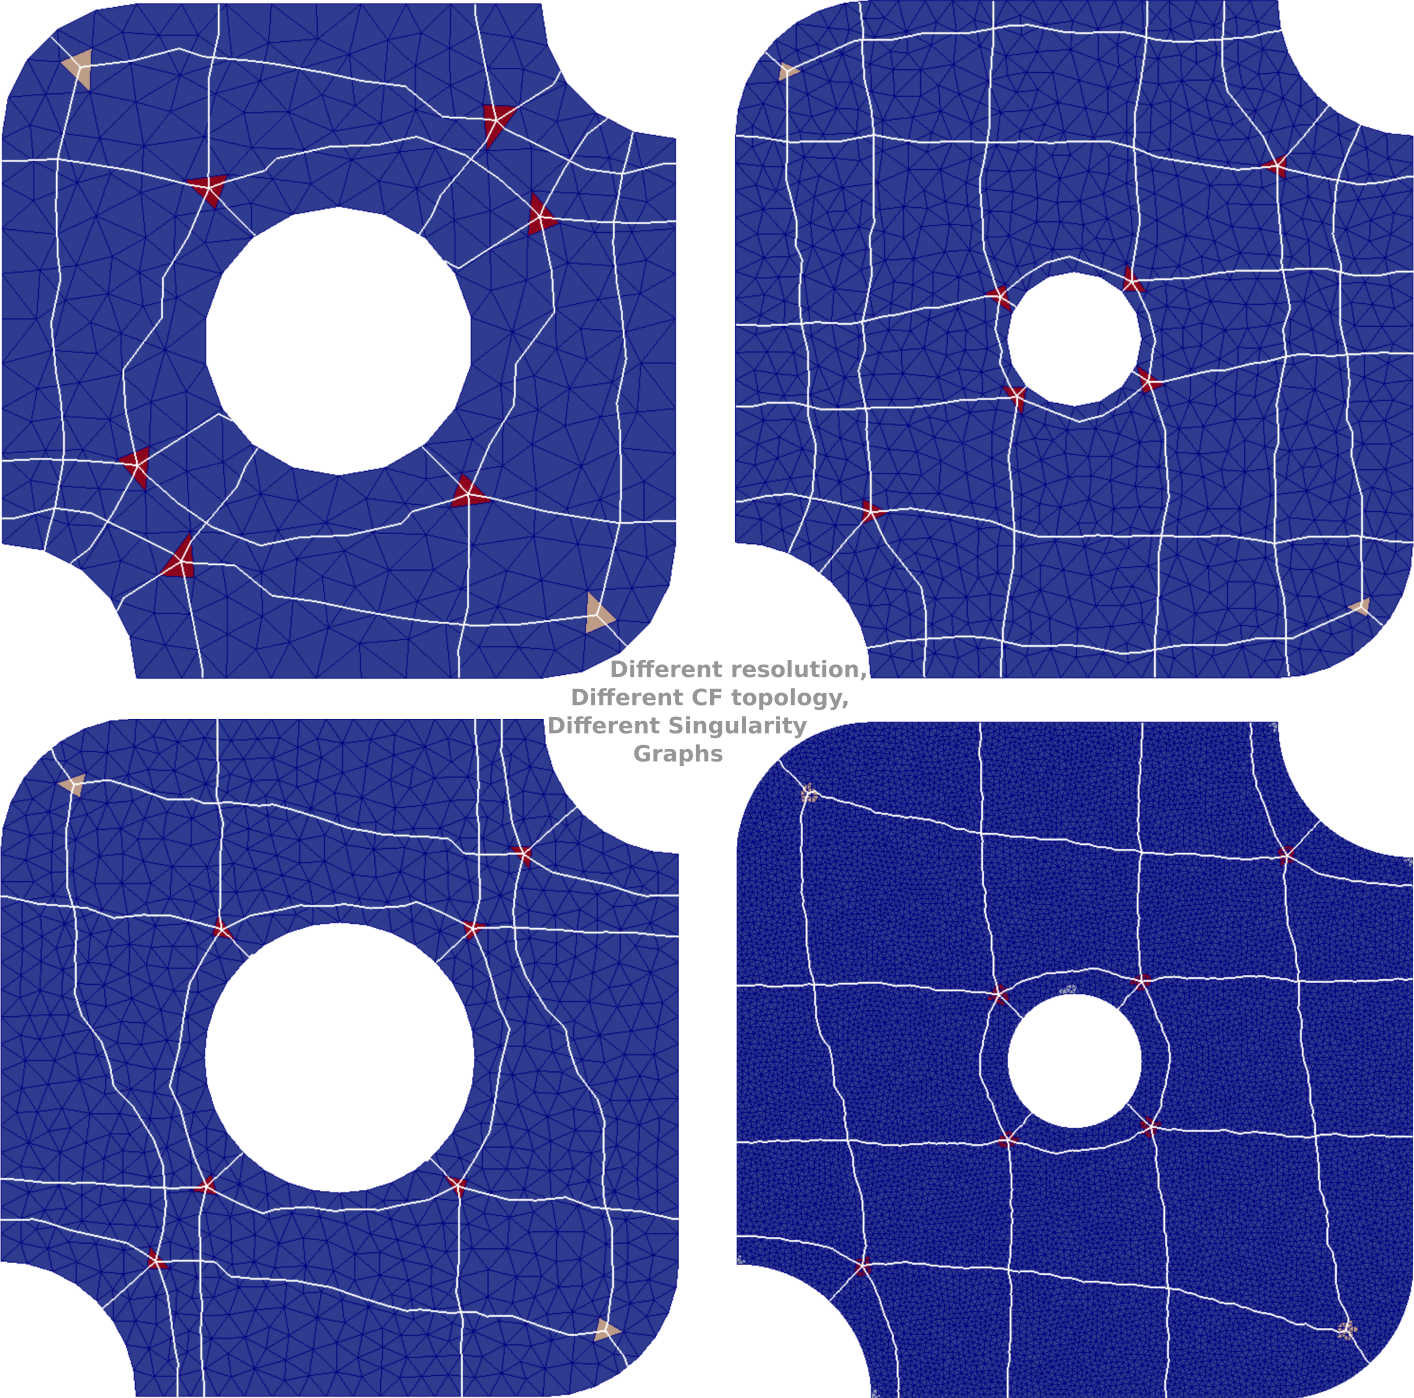
\includegraphics[width=\textwidth]{diff_res_diff_CFTop_diff_singGraph}
  \captionof{figure}{Different singularity locations}
\end{minipage}
%%%%%%%%%%%%%%%%%%%%%%%%%%%%%%%%%
\begin{minipage}[b]{0.48\linewidth}
  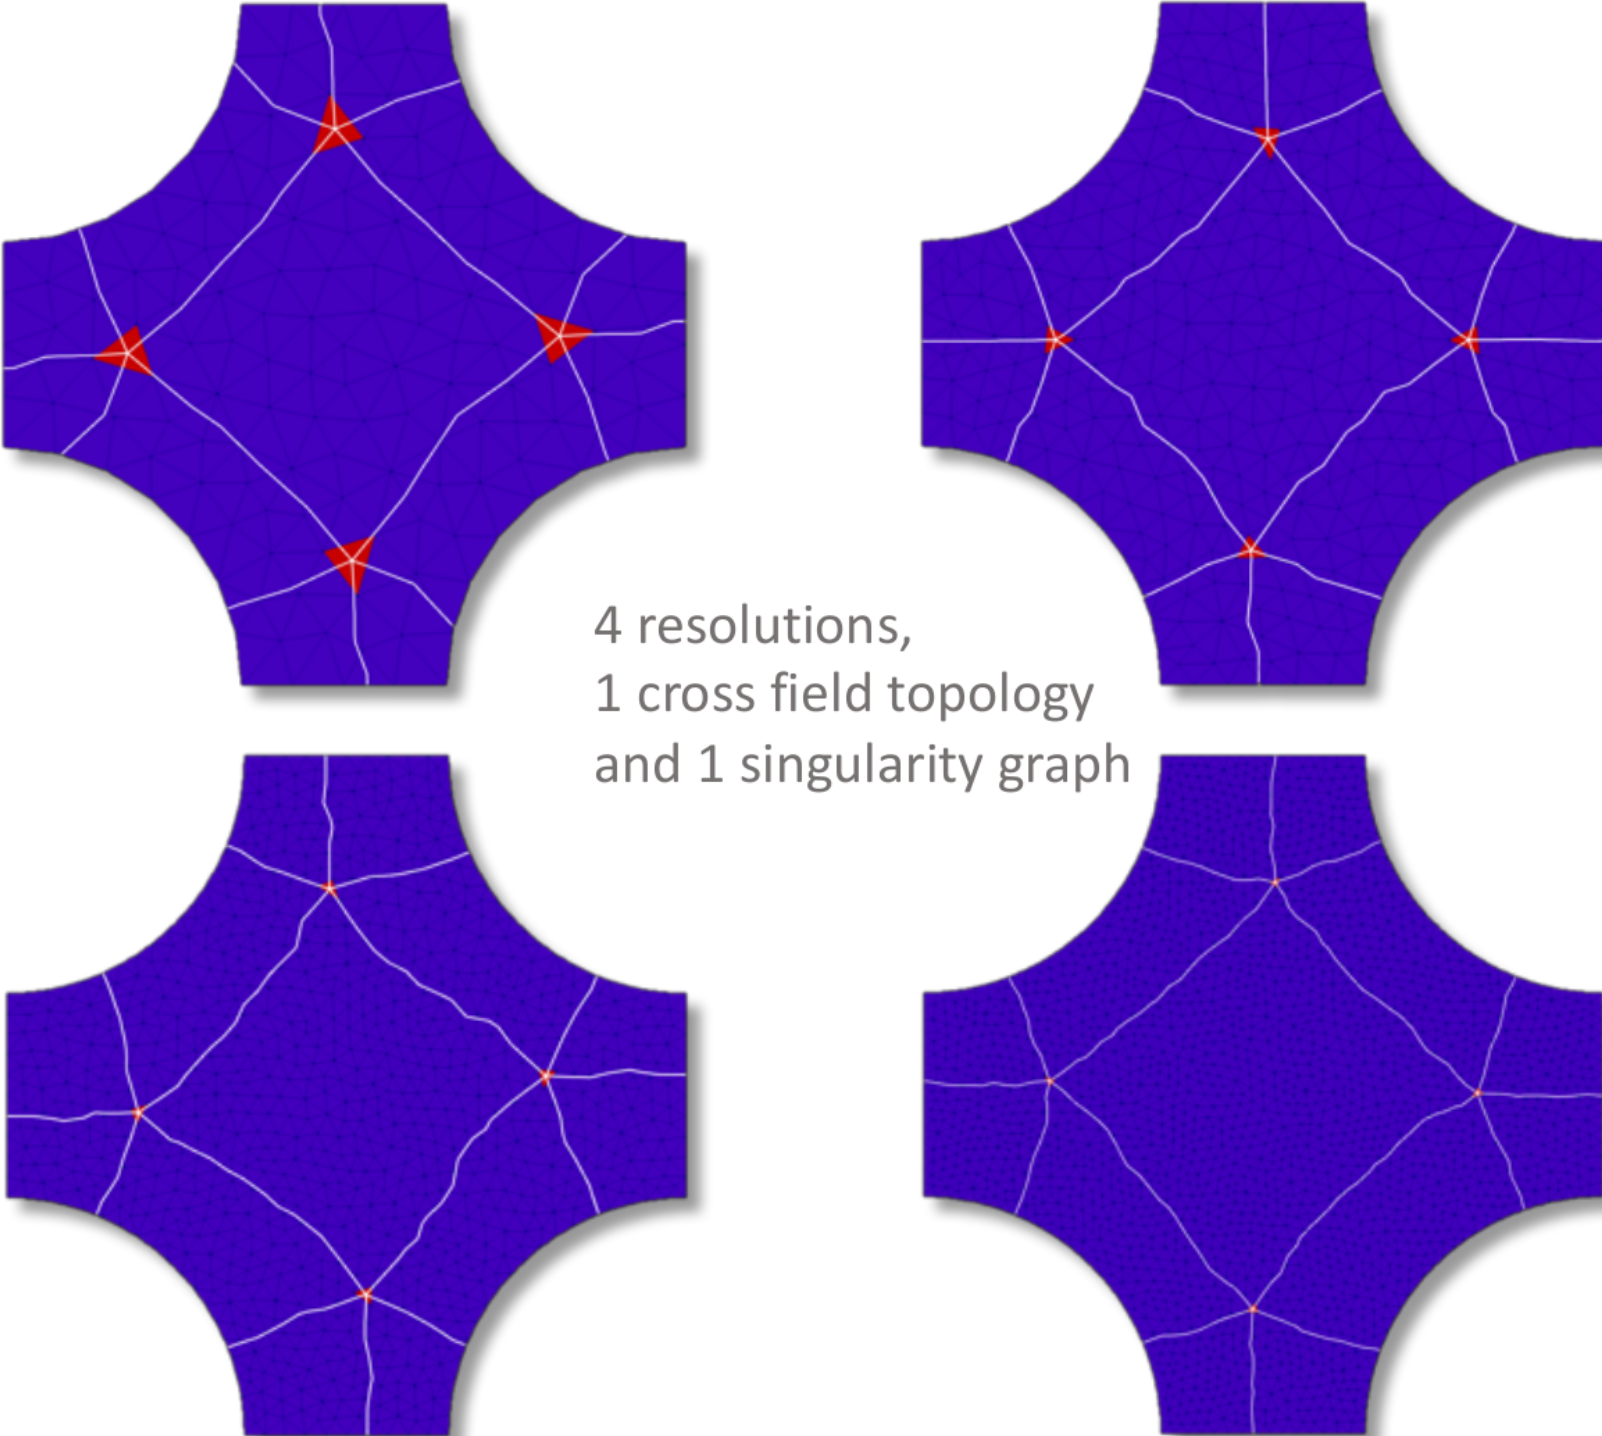
\includegraphics[width=\textwidth]{P_collection}
  \captionof{figure}{Singularities in close-to-same locations}
\end{minipage}
%%%%%%%%%%%%%%%%%%%%%%%%%%%%%%%%%
\begin{minipage}[b]{0.58\linewidth}
  \includegraphics[width=\textwidth]{O_img}
  \captionof{figure}{Different singularity locations}
\end{minipage}
%%%%%%%%%%%%%%%%%%%%%%%%%%%%%%%%%
\begin{minipage}[b]{0.38\linewidth}
  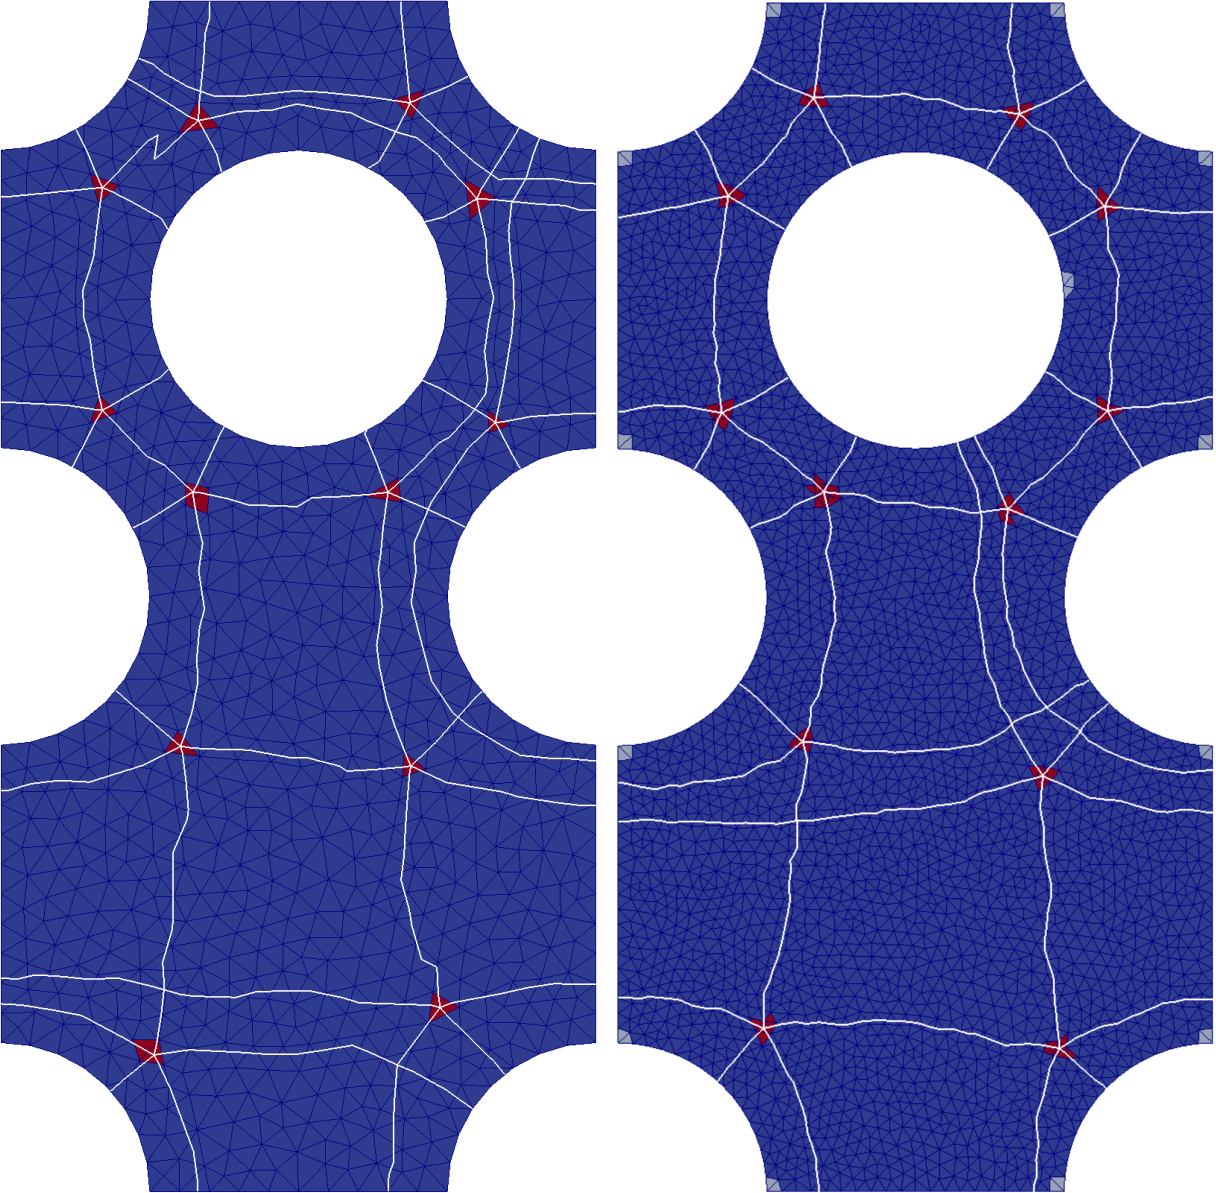
\includegraphics[width=\textwidth]{Q_img}
  \captionof{figure}{Different singularity locations}
\end{minipage}
%%%%%%%%%%%%%%%%%%%%%%%%%%%%%%%%%
%\begin{minipage}[b]{0.48\linewidth}
%  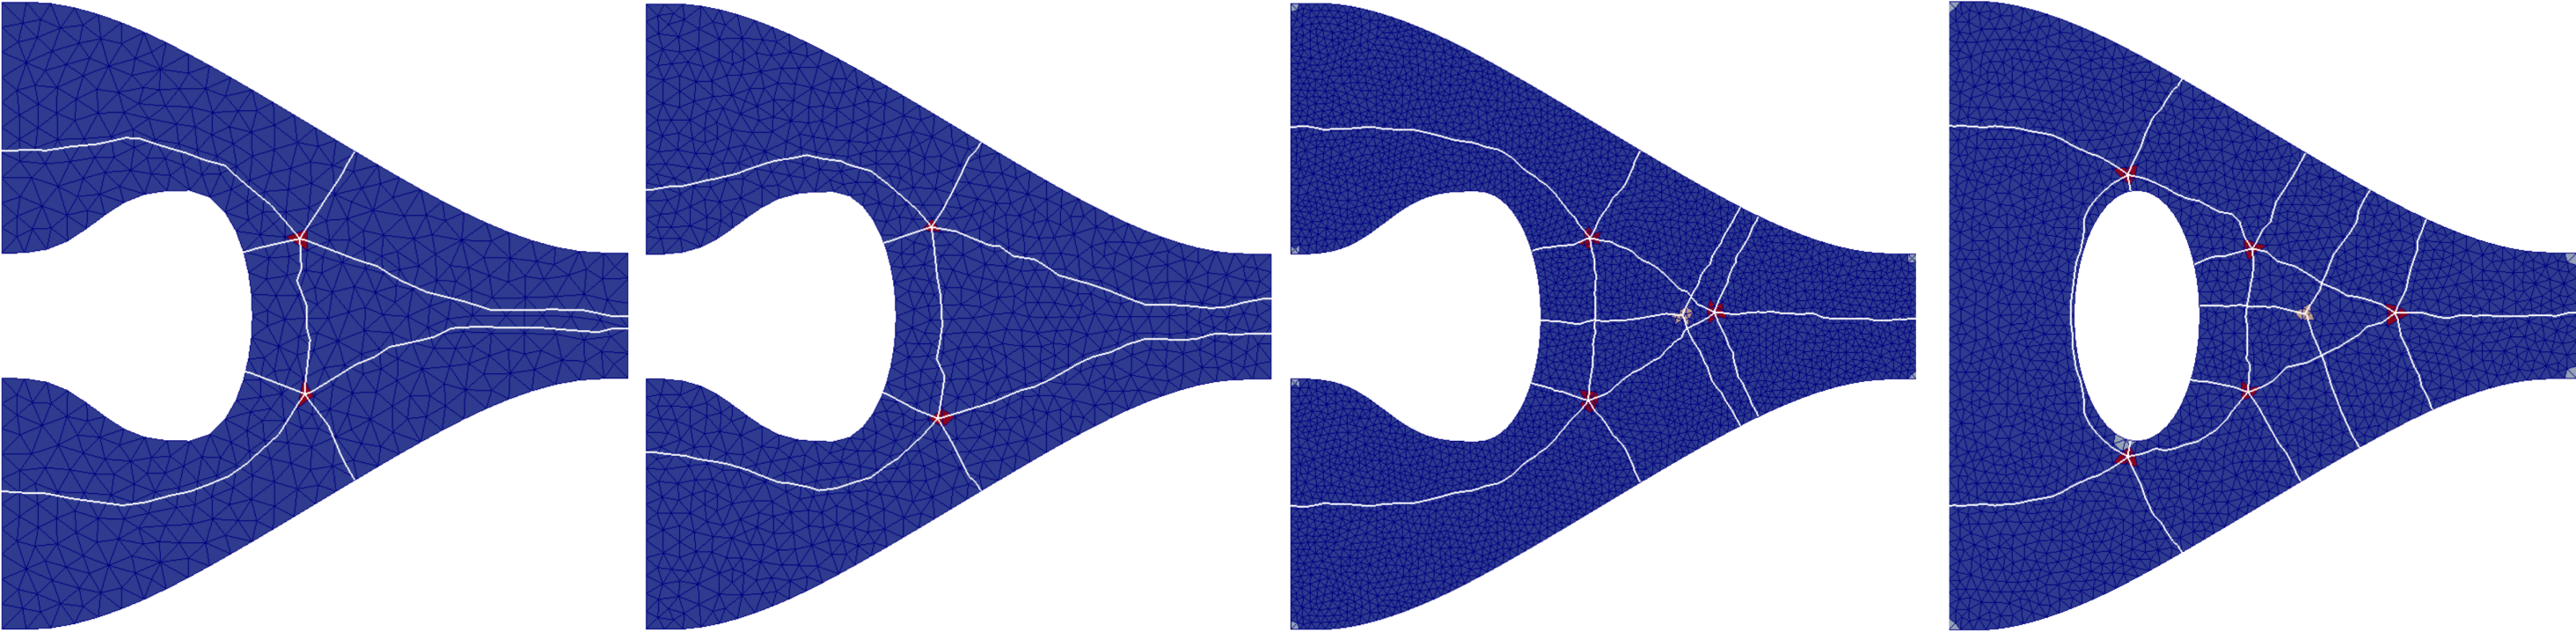
\includegraphics[width=\textwidth]{K_img}
%  \captionof{figure}{Different singularity locations}
%\end{minipage}
}
%----------------------------------------------------------------------------------------
%	Results
%----------------------------------------------------------------------------------------
%%%%%%%%%%%%%%%%%%%%%%%%%%%%%%%%%%%%%%%%%%%%%%%%%%%%%%%%%%%%%%%%%%%%%
%\headerbox{Results}{name=results,column=1,below=experimentation}{
%%%%%%%%%%%%%%%%%%%%%%%%%%%%%%%%%%%%%%%%%%%%%%%%%%%%%%%%%%%%%%%%%%%%%
%\captionsetup{labelformat=empty}
%\begin{center}
%	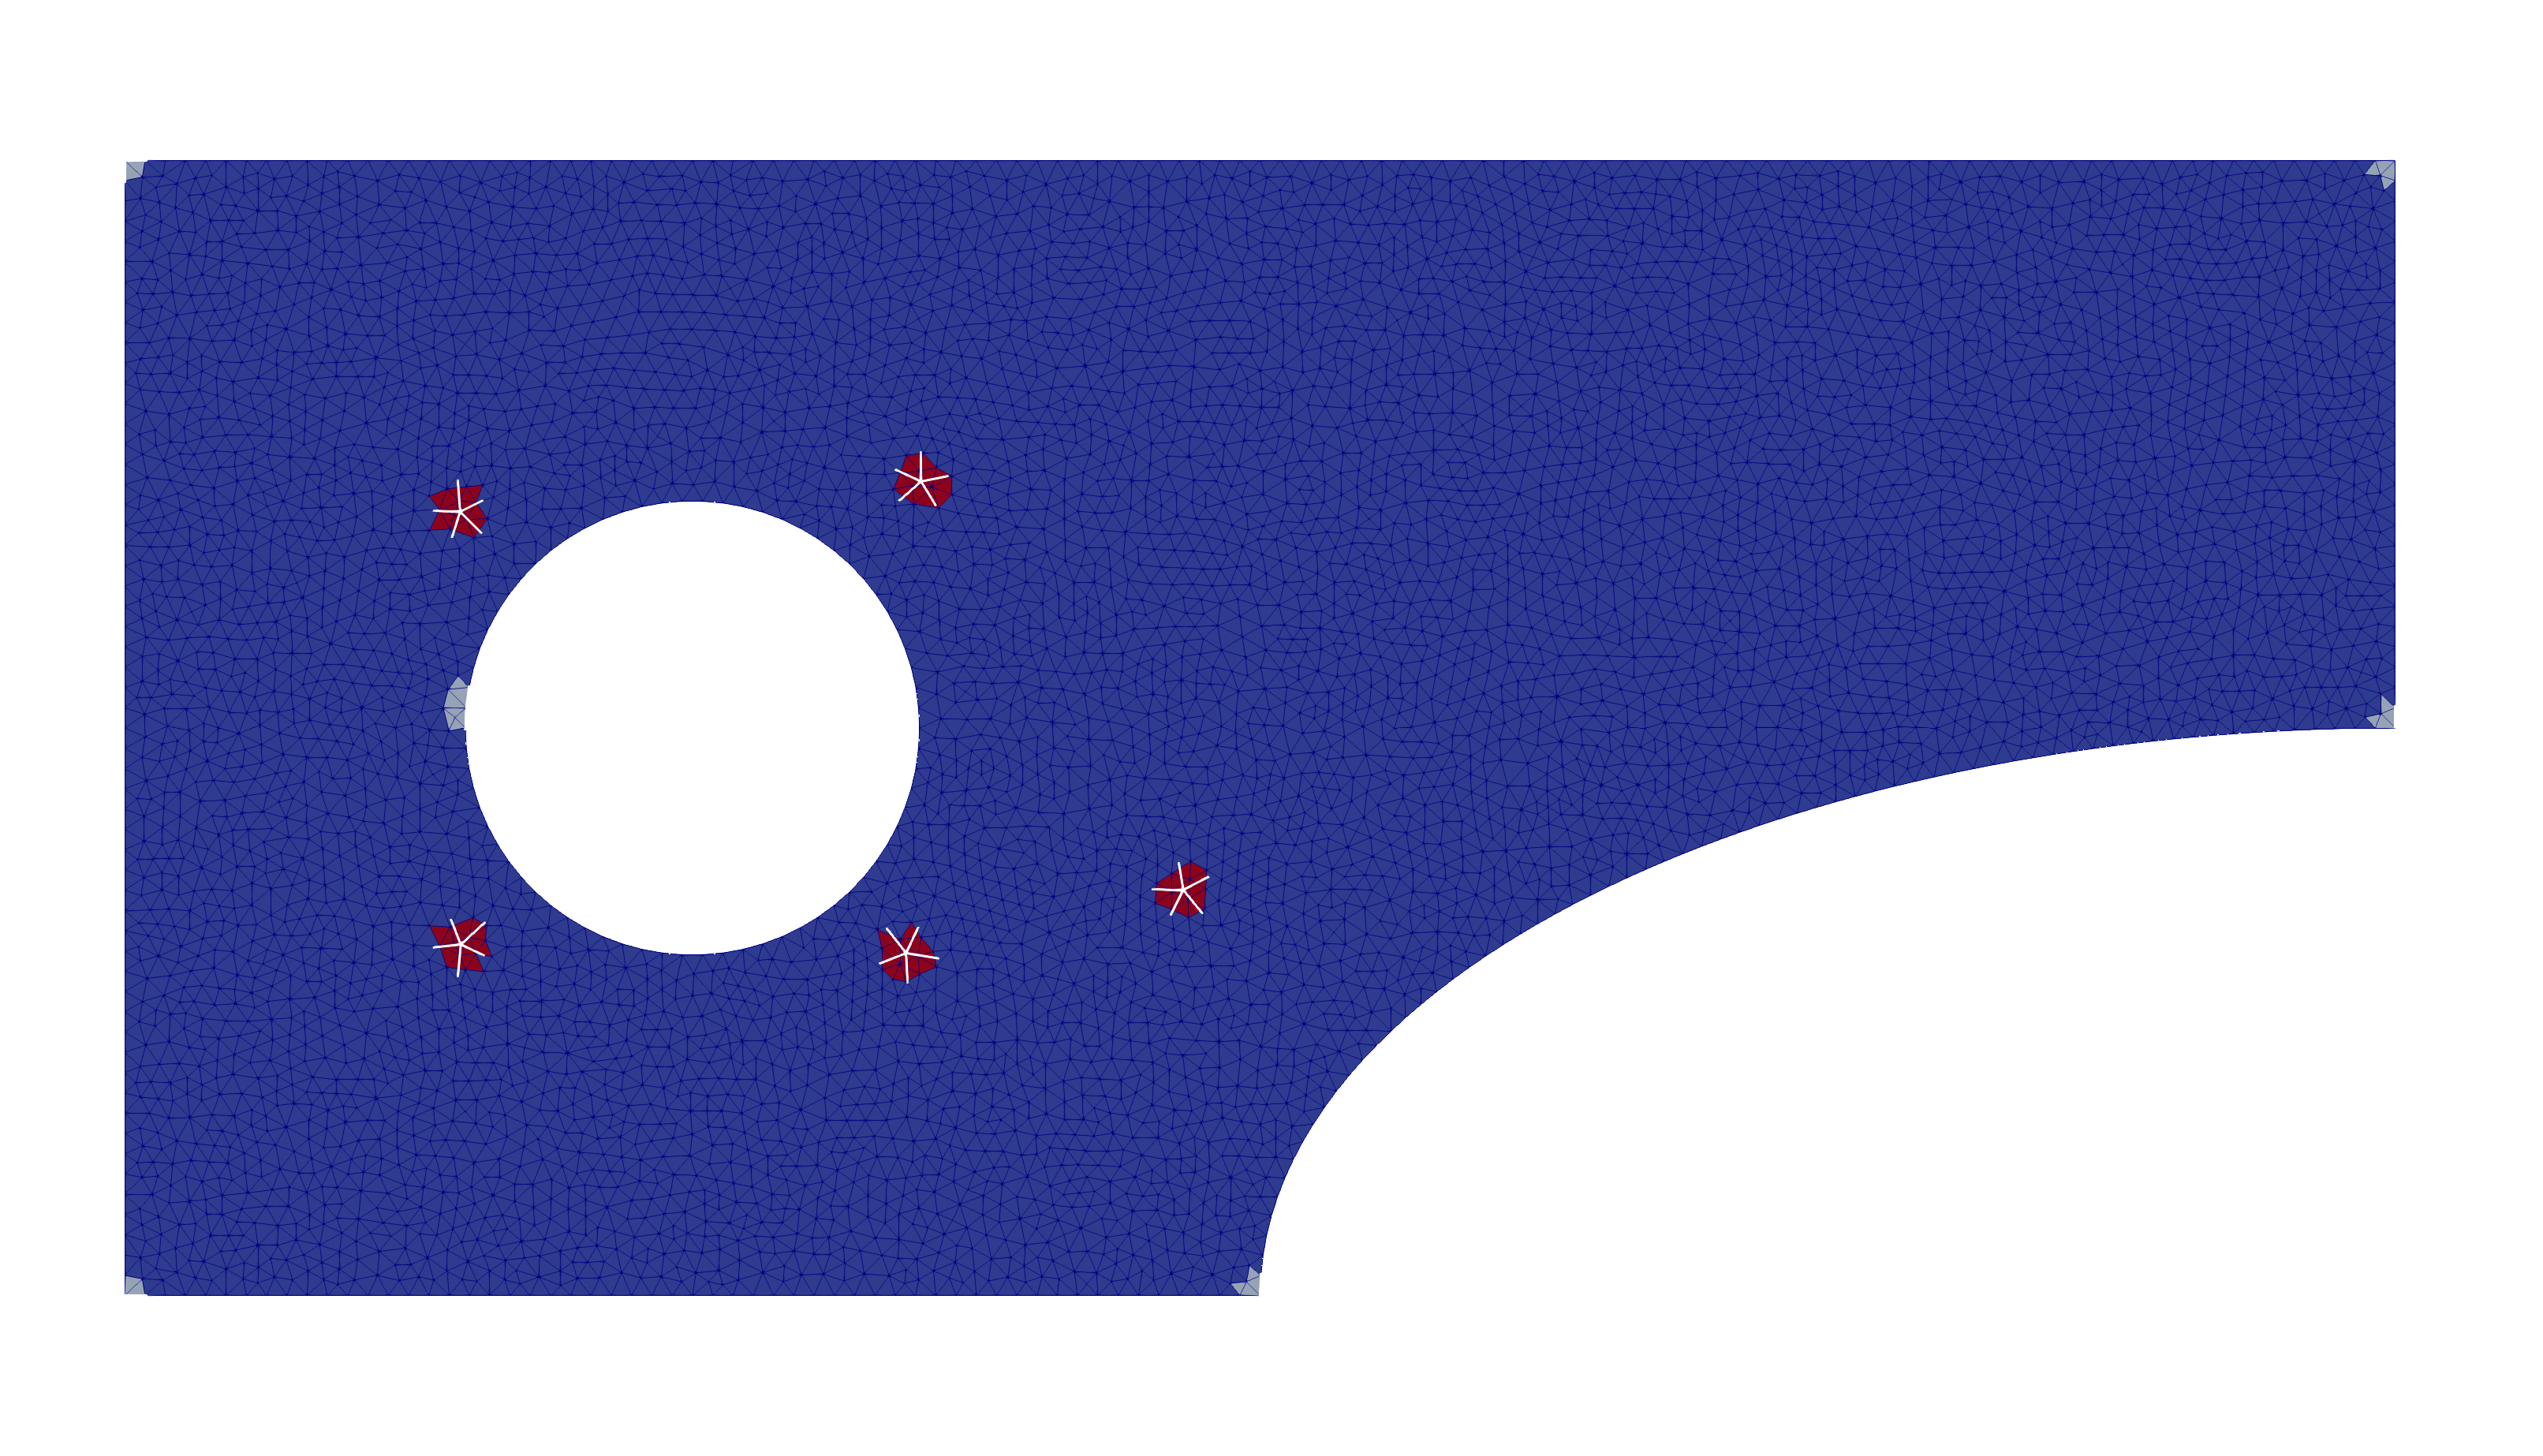
\includegraphics[height=3.7cm]{sing_slots}
%\end{center}
%\captionof{figure}{dfdgd}

%\begin{itemize}

%	\item \textbf{Proposed Solutions}

%	\item Tbbbr

%\end{itemize}
%\smallskip
%}
%----------------------------------------------------------------------------------------
%	Expected contribution and Impact
%----------------------------------------------------------------------------------------
%%%%%%%%%%%%%%%%%%%%%%%%%%%%%%%%%%%%%%%%%%%%%%%%%%%%%%%%%%%%%%%%%%%%%
%\headerbox{Conclusions and Perspectives}{name=conclusion,column=1,below=experimentation}{
%%%%%%%%%%%%%%%%%%%%%%%%%%%%%%%%%%%%%%%%%%%%%%%%%%%%%%%%%%%%%%%%%%%%%
%\medskip
%
%\smallskip
%\begin{itemize}
%\item Continuous strategies 
%\newline
% - better CF approximation (used methods: Heun or RK4)
% \newline
% - depend on proximity parameter and does not always find a valid result
% \newline
% - influence of mesh resolution - not obvious
% \newline
%\item Discrete strategy
%\newline 
%- guaranteed to find a result (importance of final choice)
%\newline
%- depends only on mesh resolution (straightforward influence: higher resolution $\rightarrow$ better approximation) 
%\item The discrete strategy is applied to the triangles of the mesh; it can be further refined by making use of the vertices as well.
%\item post-process for discrete strategy: refine detected streamlines using a continuous approach 
%\end{itemize}
%\smallskip
%}
\headerbox{Conclusions and Perspectives}{name=conclusion,column=0,row=0,span=2,above=bottom}{
\vspace{-0.1cm}\noindent
\begin{minipage}[HT!]{0.62\linewidth}
\begin{tcolorbox}[colframe=gray,boxrule=0.01pt,left=0mm,right=0mm,title=\Large Conclusions]
\vspace{-0.2cm}
  %$\ \ \ \ \ \ \ \bullet $ \textbf{Continuous strategies} 
%\noindent
%\newline
 - Continuous strategies : Improvement of the iterative strategy and implementation of the simultaneous one.
 \newline
 %- Improvement for the CF approximation (used methods: Heun or RK4).
 %\newline
 - Implementation of the discrete strategy: guaranteed to find a result, straightforward influence of the mesh resolution.%(importance of final choice);
 \newline
 - \footnotesize \textcolor{lightblue}{[Ledoux 2019]} F. Ledoux, \textit{Bringing frame field from research to industrial usage}, FRAMES 2019, First Workshop on Frame-based hex meshing, Université catholique de Louvain, Louvain-la-Neuve, July 1-2, 2019, Belgium.
  \newline
 - \footnotesize \textcolor{lightblue}{[Vintescu et al. 2019]} A.M. Vintescu and F. Ledoux, \textit{Surface Quad Blocking Using Frame Fields and Mesh Adaptation}, 15th U.S. National Congress on Computational Mechanics, July 28 - August 1, 2019, Texas USA.
   %: higher resolution $\rightarrow$ better approximation
 %\newline
 %- depend on proximity parameters and do not always find a valid result
 %\newline
 %- influence of mesh resolution - not obvious 
% $\ \ \ \ \ \ \ \bullet $ \textbf{Discrete strategy}
\vspace{-0.2cm}
\end{tcolorbox}
\vspace{-0.2cm}
\end{minipage}
\hspace{0.005\linewidth}
\begin{minipage}[HT!]{0.37\linewidth}
\begin{tcolorbox}[colframe=gray,boxrule=0.005pt,left=0mm,right=0mm,title=\Large Perspectives]
%$\ \ \ \ \ \ \ \bullet $ The strategy is applied to a graph with the nodes as the original triangle centers; it can be further refined by encompassing the vertices as well.
%\newline
%$\ \ \ \ \ \ \ \bullet $ Post-process procedure: refine the detected streamlines using a continuous approach. 
%\newline
\noindent
- Adapt the algorithm in order to obtain curve quads and automate their generation.
\newline
- Article in preparation to submit at journals JCP or Advances in Software Engineering.
\end{tcolorbox}
\end{minipage}
}
%----------------------------------------------------------------------------------------
%	References
%----------------------------------------------------------------------------------------
%%%%%%%%%%%%%%%%%%%%%%%%%%%%%%%%%%%%%%%%%%%%%%%%%%%%%%%%%%%%%%%%%%%%%
%\headerbox{References}{name=refs,column=1,below=results,above=bottom}{
%%%%%%%%%%%%%%%%%%%%%%%%%%%%%%%%%%%%%%%%%%%%%%%%%%%%%%%%%%%%%%%%%%%%%
%\renewcommand{\section}[2]{\vskip 0.05em} % Get rid of the default "References" section title
%\bibliographystyle{unsrt}
%\bibliography{biblio_hpcs} % Use sample.bib as the bibliography file
%}
%----------------------------------------------------------------------------------------
\end{poster}
\end{document}
